\chapter{Обзор исследований накопления изотопов водорода в материалах ОПЭ}\label{ch:ch1}

\nomenclature[A, 0]{УТС}{Управляемый термоядерный синтез}
\nomenclature[A, 1]{ТЯУ}{Термоядерная установка}
\nomenclature[A, 2]{ИТЭР}{Международный экспериментынй термоядерный реактор}
\nomenclature[A, 3]{ОПЭ}{Обращенные к плазме элементы}
\nomenclature[A, 4]{DT-плазма}{Дейтерий-тритиевая плазма}
\nomenclature[A, 5]{H-мода}{Режим с высоким временем удержанием энергии в плазме токамака (High confinement regime)}
\nomenclature[A, 6]{ЛИД}{Лазерно-инудуцированная десорбция}

Исследования в области управляемого термоядерного синтеза (УТС) с магнитным удержанием плазмы достигли важного этапа, на котором длительное ($\sim100-\SI{1000}{\second}$) удержание энергии в горячей плазме становится все более реализуемо. Инженерно-техническая реализация термоядерных установок (ТЯУ) промышленного масштаба потребует решения совокупности взаимосвязанных задач для осуществления квазистационарного режима горения плазмы с параметрами, необходимыми для протекания реакции термоядерного синтеза. Ключевым аспектом продолжительной работы установок такого типа являются процессы взаимодействия пристеночной плазмы с поверхностью обращенных к плазме элементов (ОПЭ)~\cite{Krieger2025}. Эти процессы существенно влияют на параметры плазмы и во многом определяют срок службы компонентов, предназначенных для защиты внутрикамерных элементов установки, что также накладывает ограничения на выбор материалов ОПЭ. Сопутствующим процессом данного взаимодействия является накопление изотопов водорода в ОПЭ. Исследование механизмов и закономерностей изотопов водорода представляет собой ключевую задачу будущих ТЯУ, использующих в качестве компонентов топлива радиоактивный тритий.

\section{Плазменные нагрузки на ОПЭ в ТЯУ}\label{sec:ch1/sec1}

% Тепловые нагрузки
Элементы первой стенки в ТЯУ на базе токамака будут подвержены воздействию интенсивных потоков тепла и частиц. В действующих установках среднее значение плотности потока тепла (отношение полной мощности, попадающей на стенку, к ее проективной площади) на ОПЭ оценивается на уровне \SIrange{0.2}{0.6}{\mega\watt\per\metre\squared}~\cite{Mazul2021}. Особенности удержания плазмы в магнитной конфигурации токамака однако приводят к появлению пространственно-временного распределения этой нагрузки. Диверторная область токамаков является наиболее нагруженной. Прогностическое моделирование для строящегося токамака ИТЭР показывает, что стационарные нагрузки в нормальных разрядах\footnote{Под <<нормальными разрядами>> подразумеваются квазистационарные режимы горения плазмы, не подверженных влиянию глобальных неустойчивостей} могут достигать величины \SIrange{5}{15}{\mega\watt\per\meter\squared}~\cite{Pitts2019,Orrico2023} вблизи пересечения сеператрисы и внешних панелей дивертора, приводя к существенному нагреву поверхности до \SIrange{500}{1000}{\kelvin}.

Величина потоков тепла на ОПЭ может меняться в ходе различных переходных процессов, которые можно разделить на медленные и быстрые. К медленным можно отнести неизбежные процессы зажигания и затухания разряда длительностью около \SI{100}{\second} для ИТЭР, а также допустимые кратковременные повышения нагрузок до уровня \SI{20}{\mega\watt\per\meter\squared} длительностью в несколько секунд~\cite{Pitts2017}. Инициирование быстрых переходных процессов связано с развитием неустойчивостей разного рода~\cite{hender2007mhd}. На рисунке~\cref{fig:ch1/Heat_loads_diagram} приведена сравнительная диаграмма тепловых потоков, приходящих на диверторные пластины ИТЭР~\cite{Linke2019}.

\begin{figure}[ht]
    \centerfloat{
        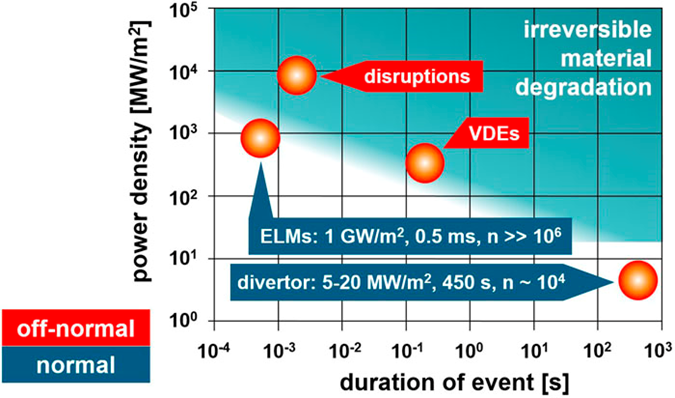
\includegraphics[scale=1]{Heat_loads_diagram.png}
    }
    \caption{Ожидаемые тепловые потоки, приходящие на ОПЭ в ИТЭР~\cite{Linke2019}. \fixme{Закрашенная} область соответствует области нанесения необратимого ущерба поверхности}\label{fig:ch1/Heat_loads_diagram}
\end{figure}

Значительную опасность представляют три типа событий: большие срывы тока, вертикальные смещения плазменного шнура и импульсно-периодические плазменные нагрузки во время ELM-событий. Большие срывы тока происходят при развитии глобальных магнитогидрониманических неустойчивостей. Они представляют наибольшую опасность, так как приводят к выбросу значительной части запасенной в плазме энергии на ОПЭ за времена порядка \SIrange{10}{100}{\milli\second}. Вертикальные смещения характерны для D-образного сечения плазменного шнура при утере устойчивости в вертикальном направлении за счет быстрых изменений параметров плазмы. События неконтролируемого вертикального смещения ведут к выходу за сепаратрису, создавая дополнительную тепловую нагрузку на ОПЭ за время порядка \SIrange{0.1}{1}{\second}. Возникновение импульсно-периодических плазменных нагрузок на ОПЭ типично для плазменных разрядов в H-моде, переход в которую сопровождается формированием транспортного барьера на периферии плазмы. Образование транспортного барьера ведет к росту давления плазмы и его градиента на периферии до тех пор, пока не будет достигнут предел магнитогидрониманической устойчивости~\cite{Leonard2014}. Возникающие в результате неустойчивости (ELM-неустойчивости) вызывают быструю релаксацию давления с выбросом потока плазмы, содержащего порядка процента запасенной энергии в плазме, на ОПЭ за время \( \sim\SIrange{0.1}{1.0}{\milli\second} \). 

Согласно оценкам~\cite{Loarte2003, hender2007mhd, Pitts2017, Pitts2019}, потоки тепла во время переходных процессов в ИТЭР могут достигать $\sim\SI{10}{\giga\watt\per\meter\squared}$. Воздействие мощных плазменных потоков во время описанных неустойчивостей может нанести серьезный ущерб поверхности (растрескивание, плавление, испарение и т.д.). Предотвращение возможного ущерба является приоритетной задачей, для решения которой разрабатываются соответствующие операционные системы и подходы~\cite{Lang2013,Evans2013,Lehnen2015}. Ввиду этого, далее в работе основное внимание будет уделено переходным процессам типа ELM-событий, последствия развития которых предполагаются либо допустимыми, либо могут быть минимизированы до приемлемого уровня.

Потоки частиц, приходящие на ОПЭ в действующих установках, в основном состоят из электронов, ионов и нейтралов перезарядки изотопов водорода. Возможно также наличие малой доли более тяжелых частиц материалов ОПЭ, остаточного газа или примесей, вводимых в установку для кондиционирования стенок или распределения тепловых нагрузок. В проектируемых ТЯУ, в т.ч. и токамаке ИТЭР, корпускулярные нагрузки также будут включать продукты DT-реакции синтеза: высокоэнергетичные нейтроны (\SI{14.1}{\mega\electronvolt}) и альфа-частицы (\SI{3.5}{\mega\electronvolt}). Длительные режимы работы установок будут сопровождаться высокой дозой облучения ОПЭ, что также может приводить к модификации как поверхностной, так и объемной структуры. К тому же, важней задачей с точки зрения обеспечения радиационной безопасности является минимизация накопления радиоактивного трития в элементах установки на протяжении ее срока эксплуатации.

Плотность потока частиц на элементы первой стенки ИТЭР оценивается на уровне \SIrange{e18}{e20}{\particles\per\metre\squared\per\second}~\cite{DeTemmerman2021, Rivals2022}, когда для диверторных пластин "--- на уровне \SIrange{e23}{e24}{\particles\per\metre\squared\per\second}~\cite{Pitts2019,Orrico2023}, причем энергия приходящих ионов составляют величину порядка \SIrange{1}{100}{\electronvolt}. Оценка суммарной дозы облучения пластин дивертора в ИТЭР показывает, что за 5000 номинальных разрядов длительностью \SI{400}{\second} ее величина составит \( \sim \SIrange{e29}{e30}{\particles\per\metre\squared} \). Как показано на сравнительных диаграммах на рисунке~\cref{fig:ch1/fluxes_comparison}, условия эксплуатации ОПЭ в ИТЭР будут намного суровее, чем в действующих установках по исследованию магнитного удержания плазмы.
\begin{figure}[ht]
    \centerfloat{
        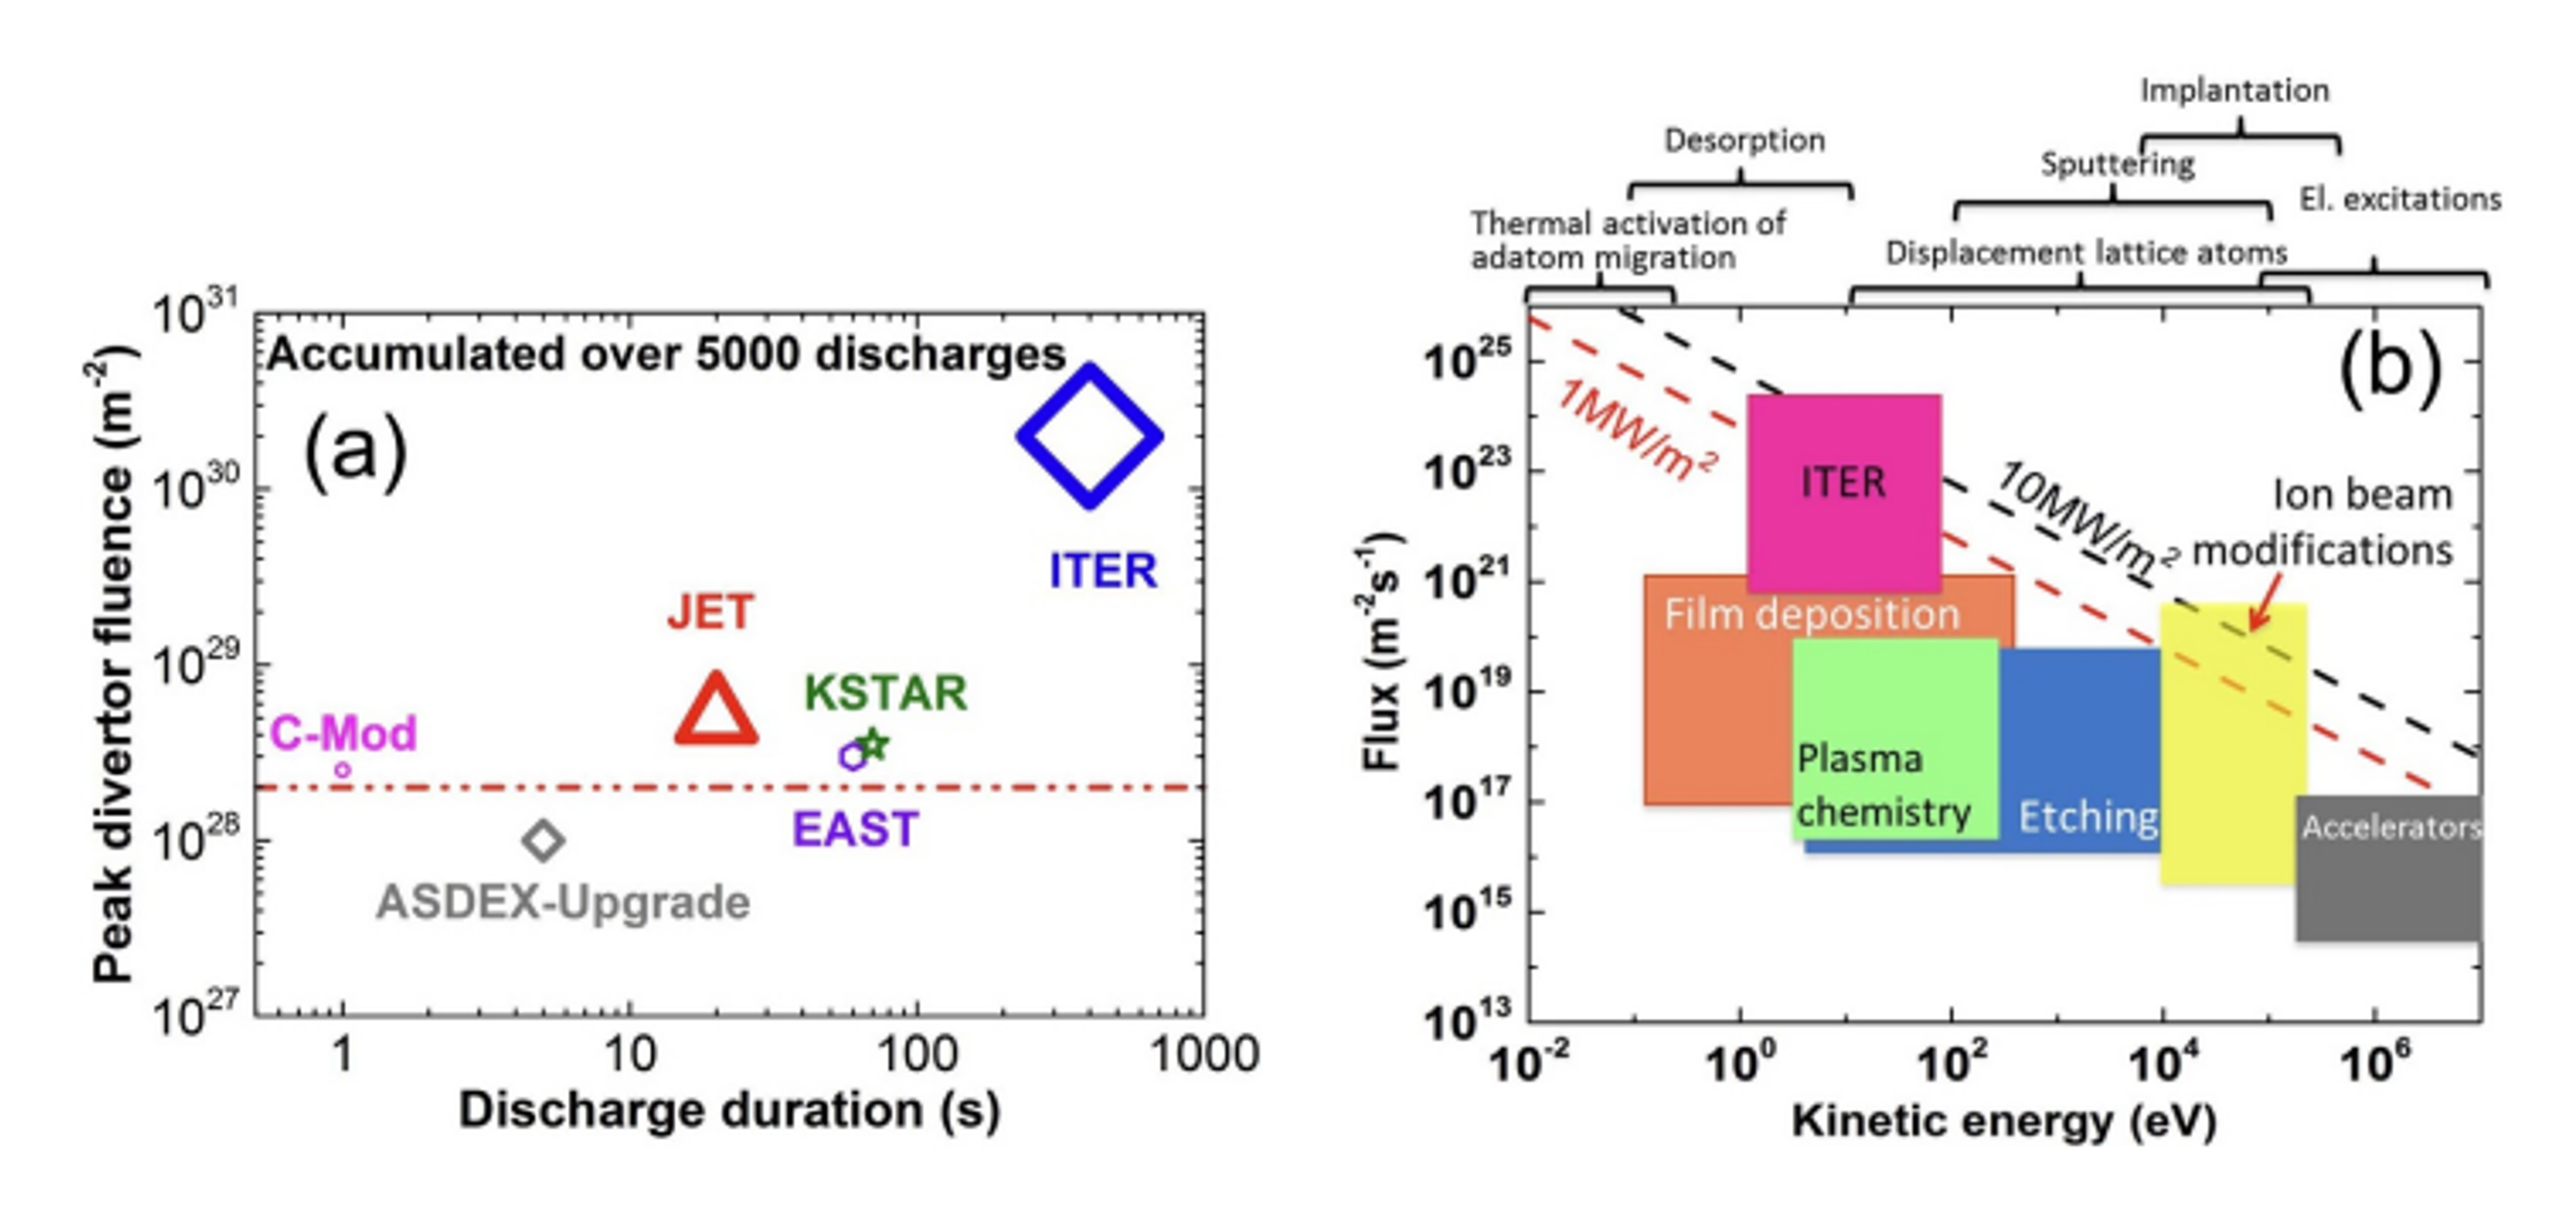
\includegraphics[scale=0.9]{fluxes_comparison.png}
    }
    \caption{Сравнение оцененной ионной дозы после 5000 тысяч нормальных плазменных разрядов в различных токамаках (слева) и характерных условий облучения в различных типах экспериментов (справа)~\cite{DeTemmerman2018}}\label{fig:ch1/fluxes_comparison}
\end{figure}
Энергии ионов в диверторе сопоставимы с энергиями, используемыми в различных методах плазменного осаждения и травления, однако плотности потока ионов и энергии на несколько порядков выше. Помимо этого, поток и энергия ионов, приходящих на поверхность ОПЭ, могут увеличиваться во время переходных процессов. Анализ данных с диагностических систем (зонды Ленгмюра и \(\mathrm{D}_\alpha\)-спектроскопия) токамака JET~\cite{Guillemaut2015,Guillemaut2018} демонстрирует кратное увеличение измерительных сигналов во время ELM-событий, что косвенно соответствуют пропорциональному росту потока частиц. Считается, что энергия частиц во время ELM-событий пропорциональна температуре плазмы на пьедестале~\cite{Eich2017}. При сохранении аналогичных зависимостей для токамака масштаба ИТЭР можно ожидать соответствующее превышение уровня стационарных нагрузок с энергия приходящих ионов порядка нескольких килоэлектронвольт.

Немаловажным остается влияние образования гелия и нейтронов на эксплуатацию ОПЭ. Генерируемы в ходе DT-реакции частицы гелия должны терять большую часть своей энергии в центре плазменного шнура, однако облучение материалов ионами гелия с низкой энергией также может оказывать существенное влияние. Известно, что облучение тугоплавких металлов ионами гелиевой плазмы индуцирует формирование гелиевых пузырей в объеме материала, а также может приводить к его структурным изменениям с образованием высокопостристых структур~\cite{Ueda2018,Kajita2018,Fedorovich2019}. Любые незапланированные структурные изменения морфологии поверхности ОПЭ будут влиять на процессы взаимодействия плазмы с ней, что может приводить к глобальным изменениям в режимах удержания плазмы.

Взаимодействие ионов с ОПЭ носит поверхностный характер. Падающий на поверхность поток частиц может приводить либо к обратной эмиссии частиц (отражение, распыление), либо к их имплантации. Средняя глубина внедрения частиц (за исключением эффектов каналирования) может достигать нескольких десятков нанометров в зависимости от состава и структуры мишени, сорта приходящих частиц и их энергии~\cite{eckstein2010penetration}. Ввиду гораздо большей глубины пробега нейтронов основные процессы взаимодействия происходят в объеме материалов. Облучение нейтронными потоками ведет к объемному нагреву материалов, трансмутации элементов, а также образованию дефектов кристаллической решетки за счет развития каскадов столкновений. Прогнозируемый уровень повреждений в конце срока службы токамака ИТЭР оценивается гораздо ниже инженерных ограничений~\cite{Villari2013}. Тем не менее, образование радиационных дефектов в материалах ОПЭ в ходе работы установки может влиять на удержание изотопов водорода.

\section{Материалы ОПЭ в ТЯУ}\label{sec:ch1/sec2}

Влияние описанных в предыдущим разделе отдельных типов нагрузок широко исследовалось в лабораторных условиях (исключением могут служить эффекты, связанные с облучением нейтронам с МэВ-ной энергии). В общем случае, они будут оказывать совместное влияние, что качественно проиллюстрировано на рисунке~\cref{fig:ch1/synergetic_diagram}. Синергетические эффекты воздействия на ОПЭ в не достижимых ранее условиях ТЯУ могут создавать новые вызовы для выбора их оптимальной конструкции.
\begin{figure}[ht]
    \centerfloat{
        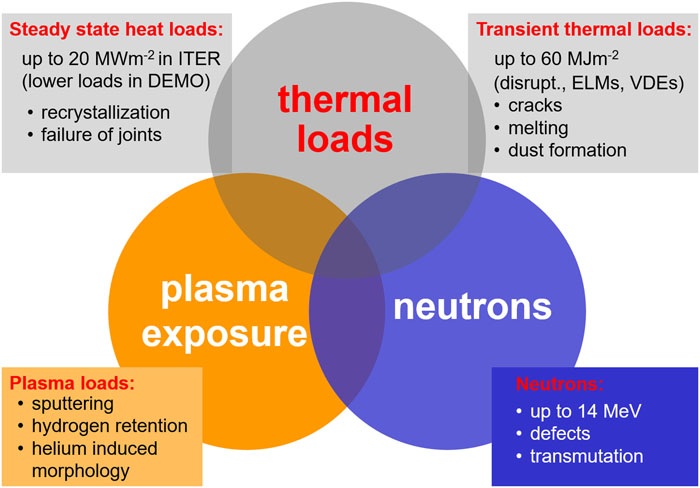
\includegraphics[scale=0.5]{synergetic_diagram.png}
    }
    \caption{Синергетические нагрузки и их основные последствия для ОПЭ при работе ТЯУ~\cite{Linke2019}}\label{fig:ch1/synergetic_diagram}
\end{figure}
Эти аспекты также накладывает совокупность требований и на выбор используемых материалов. К основным факторам, определяющим этот выбор, можно отнести термостойкость и теплопроводность, эрозионную устойчивость при ионном облучении, способность накапливать изотопов водорода, устойчивость и низкую активируемость при нейтронном облучении. Высокая термостойкость и теплопроводность, а также низкая эрозия при облучении легкими ионами характерны для тугоплавких металлов с большим зарядовым числом ядра ($Z$). Однако распыление и попадание в область горячей плазмы атомов таких материалов может приводить к увеличению потерь мощности на излучение из плазмы~\cite{Ptterich2019}. Более легкие материалы подвержены большей эрозии поверхности и могут влиять на динамику накопления изотопов водорода в ТЯУ. Основными материалами, применяемыми в современных установках, являются графит (JT-60SA~\cite{Shirai2024}, T-15МД~\cite{Velikhov2024}), бериллий (JET~\cite{Maggi2024,Kappatou2025}), молибден(EAST~\cite{Gong2024}) и вольфрам (JET, EAST, WEST~\cite{Shi2025}, ASDEX-Upgrade~\cite{Rohde2009}). 
\nomenclature[P, 01]{$Z$}{Атомный номер элемента}

Углеродные материалы являются привлекательным выбором для ОПЭ ввиду ряда преимуществ. Проникновение углерода в плазму ведет к малым потерям мощности с излучением из-за его низкого зарядового числа ($Z=6$). Углеродные материалы характеризуются высокими теплостойкостью и значением теплопроводности ($\SIrange{100}{300}{\watt\per\meter\squared\per\kelvin}$ при комнатной температуре~\cite{Merola2004, Begrambekov2023}), сопоставимой с металлами. Помимо этого, нагрев поверхности до высоких температур (>\SI{3800}{\kelvin}) ведет к сублимации материала, а не плавлению, что предотвращает вероятность развития процессов взаимодействия расплава с приповерхностной плазмой и магнитным полем. Однако углеродные материалы более подвержены распылению при облучению легкими ионами, чем, например вольфрам. а также характеризуются высоким коэффициентом химического распыления при облучении изотопами водорода. Для сравнения на рисунке~\cref{fig:ch1/sputerring_yields} приведены расчетные коэффициенты распыления углерода (физического и химического), бериллия и вольфрама. Влияние химического распыления может быть минимизировано обеспечением <<благоприятного>> режима облучения, но другим важным недостатком углеродных материалов является накопление изотопов водорода. Изотопы водорода образуют прочные C-H связи, что может приводить к чрезмерному накоплению трития в переосажденных пленках и затруднять извлечению трития из установки~\cite{Gasparyan2024}. Помимо этого, интенсивное облучение потоками нейтронов и компонентов плазмы может приводить к деградации теплофизических свойств~\cite{Wu1994} и структурным изменениям поверхностных слоев~\cite{Wang2018,Begrambekov2019,Seyedhabashi2025}.

\begin{figure}[ht]
    \centerfloat{
        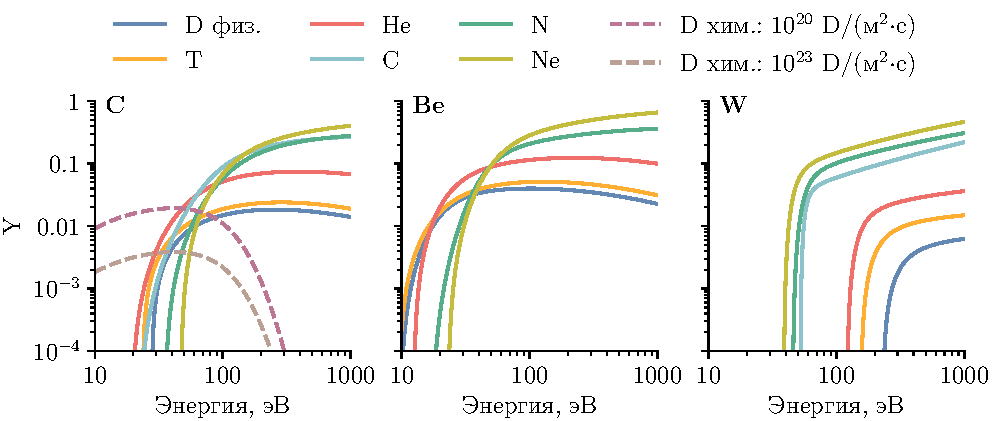
\includegraphics[scale=1]{sputerring_yields.pdf}
    }
    \caption{Расчетные зависимости коэффициентов физического распыления бериллия, углерода и вольфрама от энергии некоторых типов ионов при нормальном падении~\cite{international2001iaea, behrisch_2025}. Для углерода также приведены зависимости коэффициента химического распыления дейтерием при комнатной температуре и различных значениях плотности потока~\cite{Roth1999,Roth2004}}\label{fig:ch1/sputerring_yields}
\end{figure}

Бериллий, как и углерод, обладает низким атомным номером ($Z=4$), что обеспечивает относительно хорошую совместимость за счет минимизации потерь мощности на излучения при проникновение бериллия в область горячей плазмы. Он также обладает высокой теплопроводностью (\SI{200}{\watt\per\meter\per\K}) и относительно высокой температурой плавления (\SI{1560}{\kelvin})~\cite{Ho1974}. По сравнению с углеродными материалами, скорость химического распыления~\cite{Brezinsek2014} и накопления изотопов водорода~\cite{DeTemmerman2021} в нем существенно меньше. Переход к металлической облицовке в токамаке JET привел к снижению интегральной эрозии ОПЭ и, как следствие, накоплению изотопов водорода в несколько раз~\cite{Brezinsek2015}. Бериллий также химически активен, что позволяет эффективно связывать кислород. Не смотря на явные преимущества бериллия как материала для ОПЭ, он обладает рядом существенных недостатков. Первым из них является токсичность бериллиевой пыли, что требует применения специальных мер по работе с ним~\cite{Strupp2011}. Вторым недостатком является низкая энергия связи атомов кристаллической решетки, что приводит к более высокому коэффициенту физического распыления по сравнению с графитом (рис.~\cref{fig:ch1/sputerring_yields}) и, соответственно, меньшему сроку службы под действием интенсивного ионного облучения. Следующим негативным свойством является деградация теплофизических свойств и охрупчивание бериллия, являющееся синергетическим эффектом облучения потоками нейтронов и гелия~\cite{Kesternich2003,Gilbert2012}. Последним является малая температура плавления по сравнению с иными материалами, что ограничивает использование бериллия в высоконагруженных областях установки без активного охлаждения. Совокупность этих и иных особенностей послужили причиной принятия решения об отказе от использования бериллия в качестве ОПЭ токамака ИТЭР~\cite{Barabaschi2025}, однако использование бериллия рассматривается для российского токамака ТРТ~\cite{Mazul2021,Piskarev2024}.

Молибден ($Z=42$) и вольфрам ($Z=74$) являются тугоплавкими металлами с высокими температурами плавления: \SI{2896}{\kelvin} и \SI{3695}{\kelvin}, соответственно. Однако вольфрам предпочтительнее по причине более высоких эксплуатационных характеристик, хоть и обладает рядом свойств усложняющих технологическое производство элементов облицовки с ним~\cite{Piskarev2024}. Исходя из этого, основное внимание будет уделено вольфраму. Помимо высокой теплостойкости, вольфрам характеризуется низким коэффициентом распыления легкими ионами (рис.~\cref{fig:ch1/sputerring_yields}), совместимостью с нейтронным облучением и низкой растворимостью изотопов водорода~\cite{Roth2011, Pintsuk2012,Rieth2019}. Явным недостатком вольфрама является вероятность распыления тяжелыми примесными ионами в плазме или ее легкими основными компонентами с высокой энергией, сопровождаемое загрязнением плазмы частицам с высоким атомным номером. Как отмечалось в разделе~\cref{sec:ch1/sec1}, потоки частиц плазмы с высокой энергией ожидаются в ходе различных переходных процессов. Известна также проблема образования трещин на поверхности вольфрама при циклических тепловых нагрузках, характерных для ELM-событий. Дополнительно необходимо отметить активно исследуемые в последнее время изменения поверхности вольфрама при облучении ионами гелиевой плазмы. В условиях, характерных для диверторной области токамаков, облучение ионами гелия ведет к формированию высокопористой наноструктуризованной морфологии, называемой <<пух>>~\cite{Ueda2018,Kajita2018,Fedorovich2019,hammond2017helium,Kajita2020,Wright2022}. Рост вольфрамового <<пуха>> на поверхности может повысить вероятность зажигания униполярных дуг с соответствующем увеличением уровня эрозии поверхности. Невзирая на недостатки вольфрама, он выбран в качестве основного материала ОПЭ для ИТЭР~\cite{Pitts2025} и находится в приоритетном списке как для ТРТ~\cite{Piskarev2024}, так и для других установок, проектируемых в настоящее время.

Учитывая риски появления тяжелой примеси в горячей плазме при распылении вольфрама, рассматривается применения различных материалов для нанесения кондиционирующих покрытий. Двумя распространенными материалами, применяемыми в действующих установках, являются бор ($Z=3$) и литий ($Z=5$). Оба материала обладают низким атомным номером и являются химически активными по отношению к кислороду и углероду, что позволяет снизить долю более тяжелой примеси в плазме~\cite{Winter1996,Wauters2020}. С другой стороны, более высокая скорость эрозии покрытий требует применения методов их регулярного обновления. Тем не менее, эксперименты на токамаках ASDEX-Upgrade~\cite{Krieger2023} и EAST~\cite{Yu2023} продемонстрировали, что применении легких материалов для кондиционирования стенок может обеспечить режимы плазменных разрядов с низким рециклингом изотопов водорода, обеспечивая достижение длительных стабильных разрядов~\cite{Zakharov2019}. Помимо методов нанесения защитных покрытий, ведется активное развитие альтернативных вариантов, например самопассивируемые сплавы вольфрама с пониженным термоокислением~\cite{Litnovsky2020} и капиллярно-пористые системы с жидкими металлами~\cite{Lublinskii2015}, которые, возможно, решат проблемы, характерные для традиционных материалов.

\section{Накопление изотопов водорода в вольфраме}\label{sec:ch1/sec3}

Как показно в предыдущем разделе, вольфрам обладает совокупностью свойств, определяющим его применимость в качестве материала ОПЭ. Перспектива его использования инициировала всестороннее изучение закономерностей накопления изотопов водорода в условиях, ожидаемых в ТЯУ. Необходимость детального анализа во многом обусловлена необходимостью контроля за содержанием радиоактивного трития. Так, для токамака ИТЭР установлен административный лимит в \SI{700}{\gram} по интегральному накоплению в элементах вакуумной камеры с учетом возможных погрешностей и накопления в крионасосах~\cite{Roth1}.

\subsection{Механизмы длительного накопления изотопов водорода в ТЯУ}\label{sec:ch1/sec3/subsec1}

Изотопы водорода могут накапливаться на поверхности ОПЭ за счет адсорбции низкоэнергетичных атомов или молекул. Совокупность каналов адсорбции является процессом динамического (краткосрочного) удержания и не представляет особой проблемы, так как дегазация поверхности протекает достаточно быстро при повышенных температурах. Выделяют два основных канала долгосрочного удержания изотопов водорода: захват в объеме материала и соосаждение~\cite{Gasparyan2024, Skinner2009}. Также можно отметить накопление изотопов на поверхности или в объеме пылевых микрочастиц, образующихся в процессе эрозии поверхностных слоев ОПЭ. Накопление в пылевых частицах сильно зависит от механизма их образования и во многом может описываться процессами, определяющими захват водорода в объеме ОПЭ или при соосаждении. В силу этого, внимание будет уделено двум другим процессам долгосрочного удержания изотопов водорода в ТЯУ.

Основные процессы, определяющие долгосрочное накопление, схематически представлены на рисунке~\cref{fig:ch1/retention_mechanisms}.
\begin{figure}[ht]
    \centerfloat{
        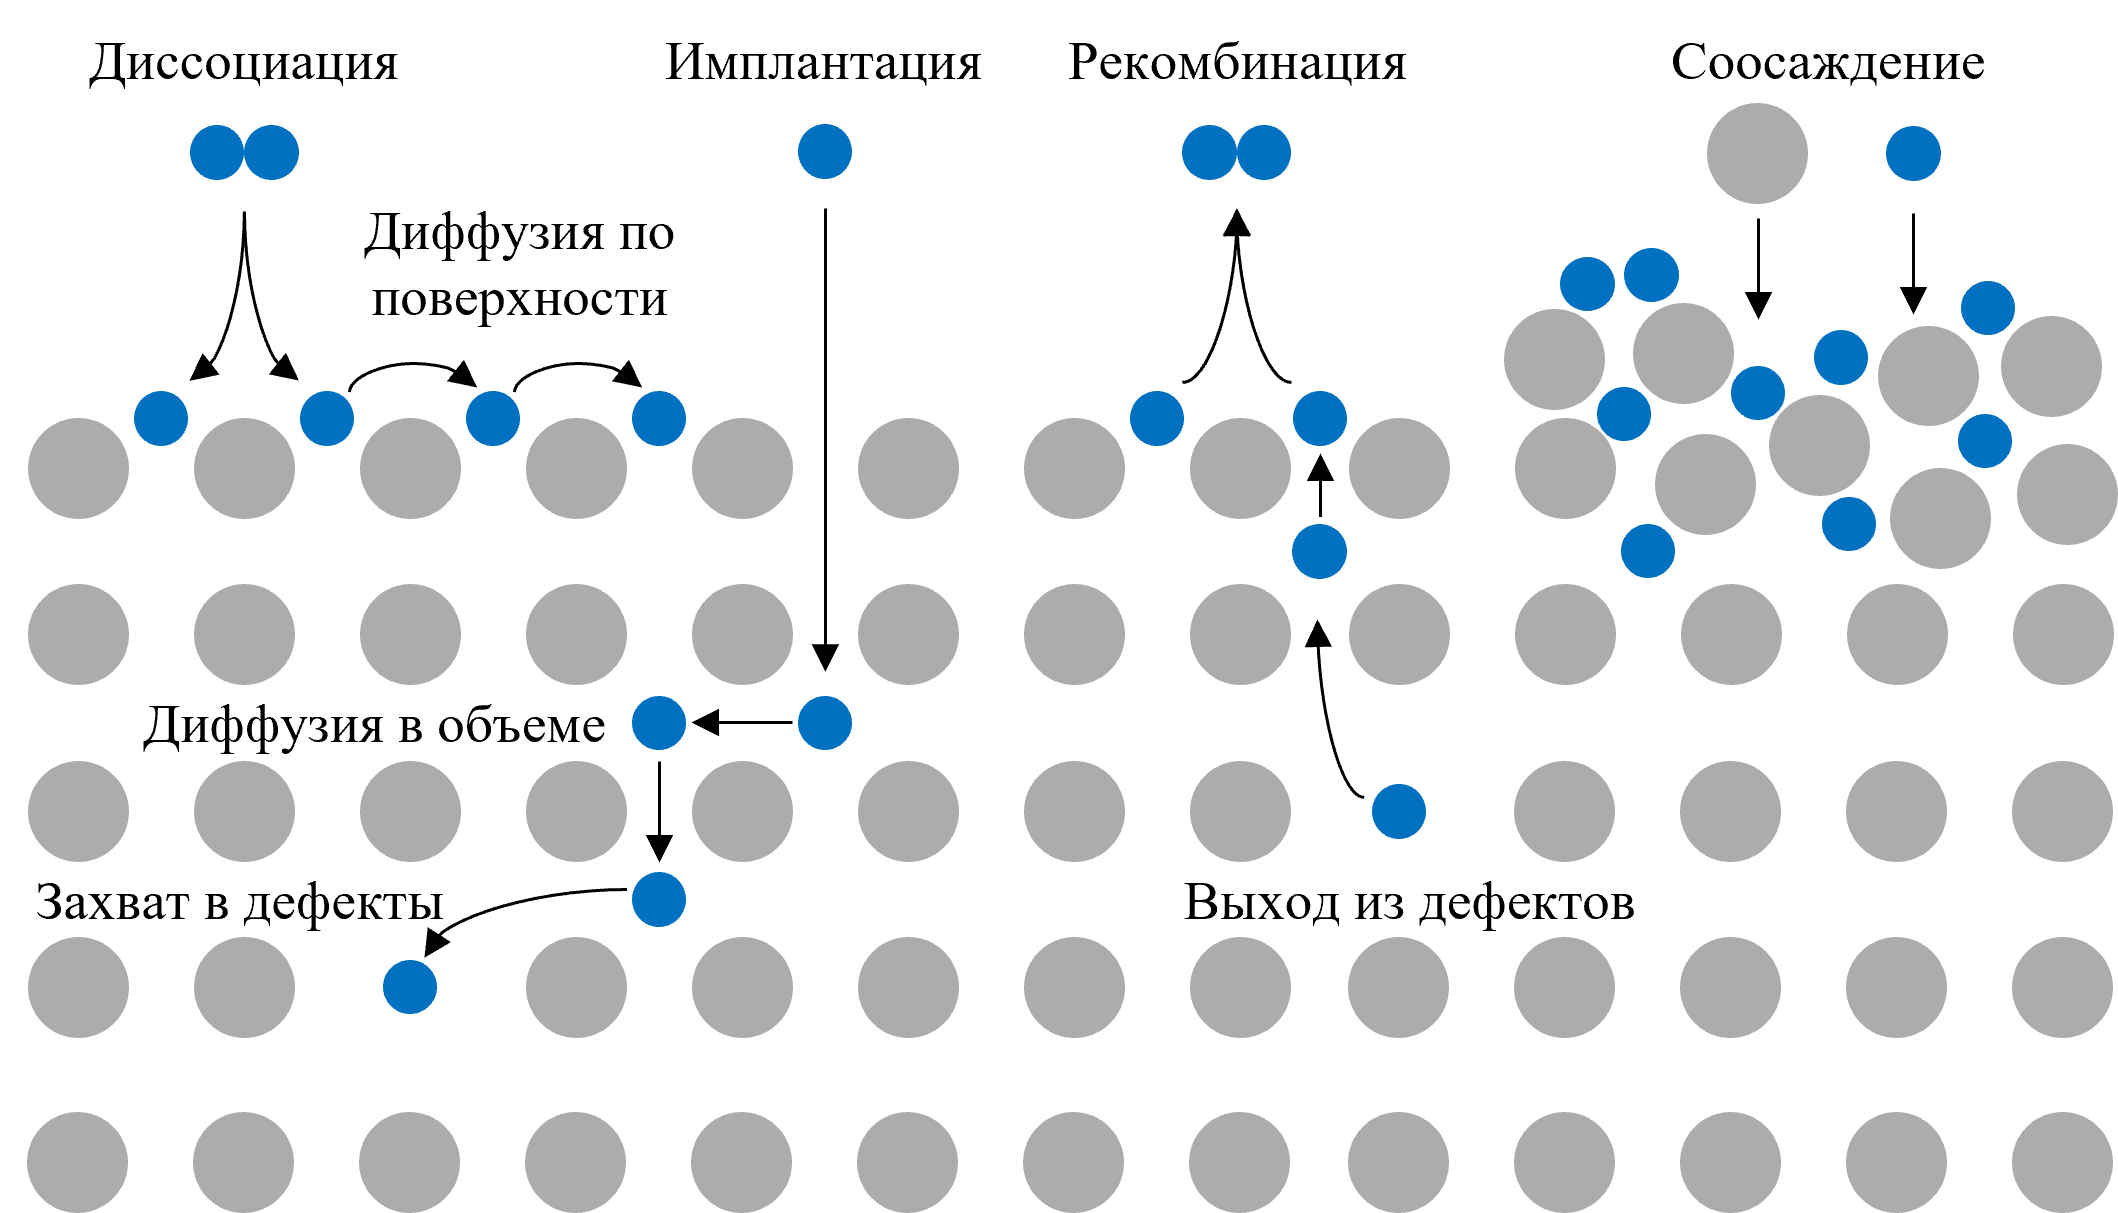
\includegraphics[scale=1]{retention_mechanisms.png}
    }
    \caption{Схематическое представление процессов захвата изотопов водорода при имплантации и соосаждении. Синие круги соответствуют атомам водорода, серые "--- атомам облучаемого материала}\label{fig:ch1/retention_mechanisms}
\end{figure}
Захват изотопов водорода при ионном облучении изначально происходит за счет имплантации частиц. Вероятность внедрения ионов определяется интегральным коэффициентом отражения, зависящим от параметров облучения и сортов взаимодействующих частиц. При попадании в объем внедренные частицы продолжают движение, теряя свою начальную энергию за счет упругих и неупругих потерь, пока не термализуются. Подвижность атомов водорода в металлах, как вольфрам, остается достаточно высокой при повышенных температурах, что позволяет им диффундировать обратно к поверхности и десорбироваться за счет различных процессов, например ассоциативной рекомбинации. С другой стороны, характерная глубина внедрения ионов в условиях токамака не превышает десятков нанометров. Интенсивное облучение поверхности приводит к быстрому насыщению водорода в зоне имплантации, что инициирует распространение водорода вглубь материала. В ходе диффузии подвижные атомы водорода могут захватываться различными дефектами кристаллической решетки, представляющие собой более глубокие потенциальные ямы по сравнению с межузельными положениями. Учитывая диффузионный характер накопления, величина интегрального накопления пропорциональна квадратному корню из времени (дозы) облучения, что наблюдается в многочисленных экспериментах~\cite{Ogorodnikova2003,Ogorodnikova2009,Sugiyama2014,Zhang2020}. Ввиду малой растворимости водорода в вольфраме, долгосрочное накопление будет определяться распределением и концентрацией дефектов, образование которых будет происходить при ионном и нейтронном облучении.

Процесс соосаждения водорода и материалов первой стенки в токамаках происходит в несколько итерационных этапов. Непрерывное распыление материалов ОПЭ приводит к попаданию примесных атомов в плазму, в которой они ионизуются. Ионы материалов стенки за счет процессов переноса в пристеночной плазме в итоге нейтрализуются и осаждаются на других элементах облицовки, инициируя рост поверхностных пленок. В то же время осаждаемые пленки подвергаются непрерывному облучению потоками частиц из плазмы. Совместное протекание обоих процессов ведет к практическому равномерному накоплению изотопов водорода, интегральная величина которого растет приблизительно линейно с временем. Важно заметить, что накопление изотопов водорода в процессе совместного соосаждения также сопровождается всеми процессами, характерными при имплантации в объем.

Результаты, полученные на современных токамаках, указывают на то, что соосаждение является доминирующим каналом накопления изотопов водорода. Параметры удержания водорода, физические свойства и скорость роста пленок сильно зависят от условий совместного осаждения~\cite{Gasparyan2019,Krat2020,Krat2025}. Доля водорода в пленках может достигать десятков процентов для различных материалов (см. Рисунок~\cref{fig:ch1/codeposition_review}).
\begin{figure}[ht]
    \centerfloat{
        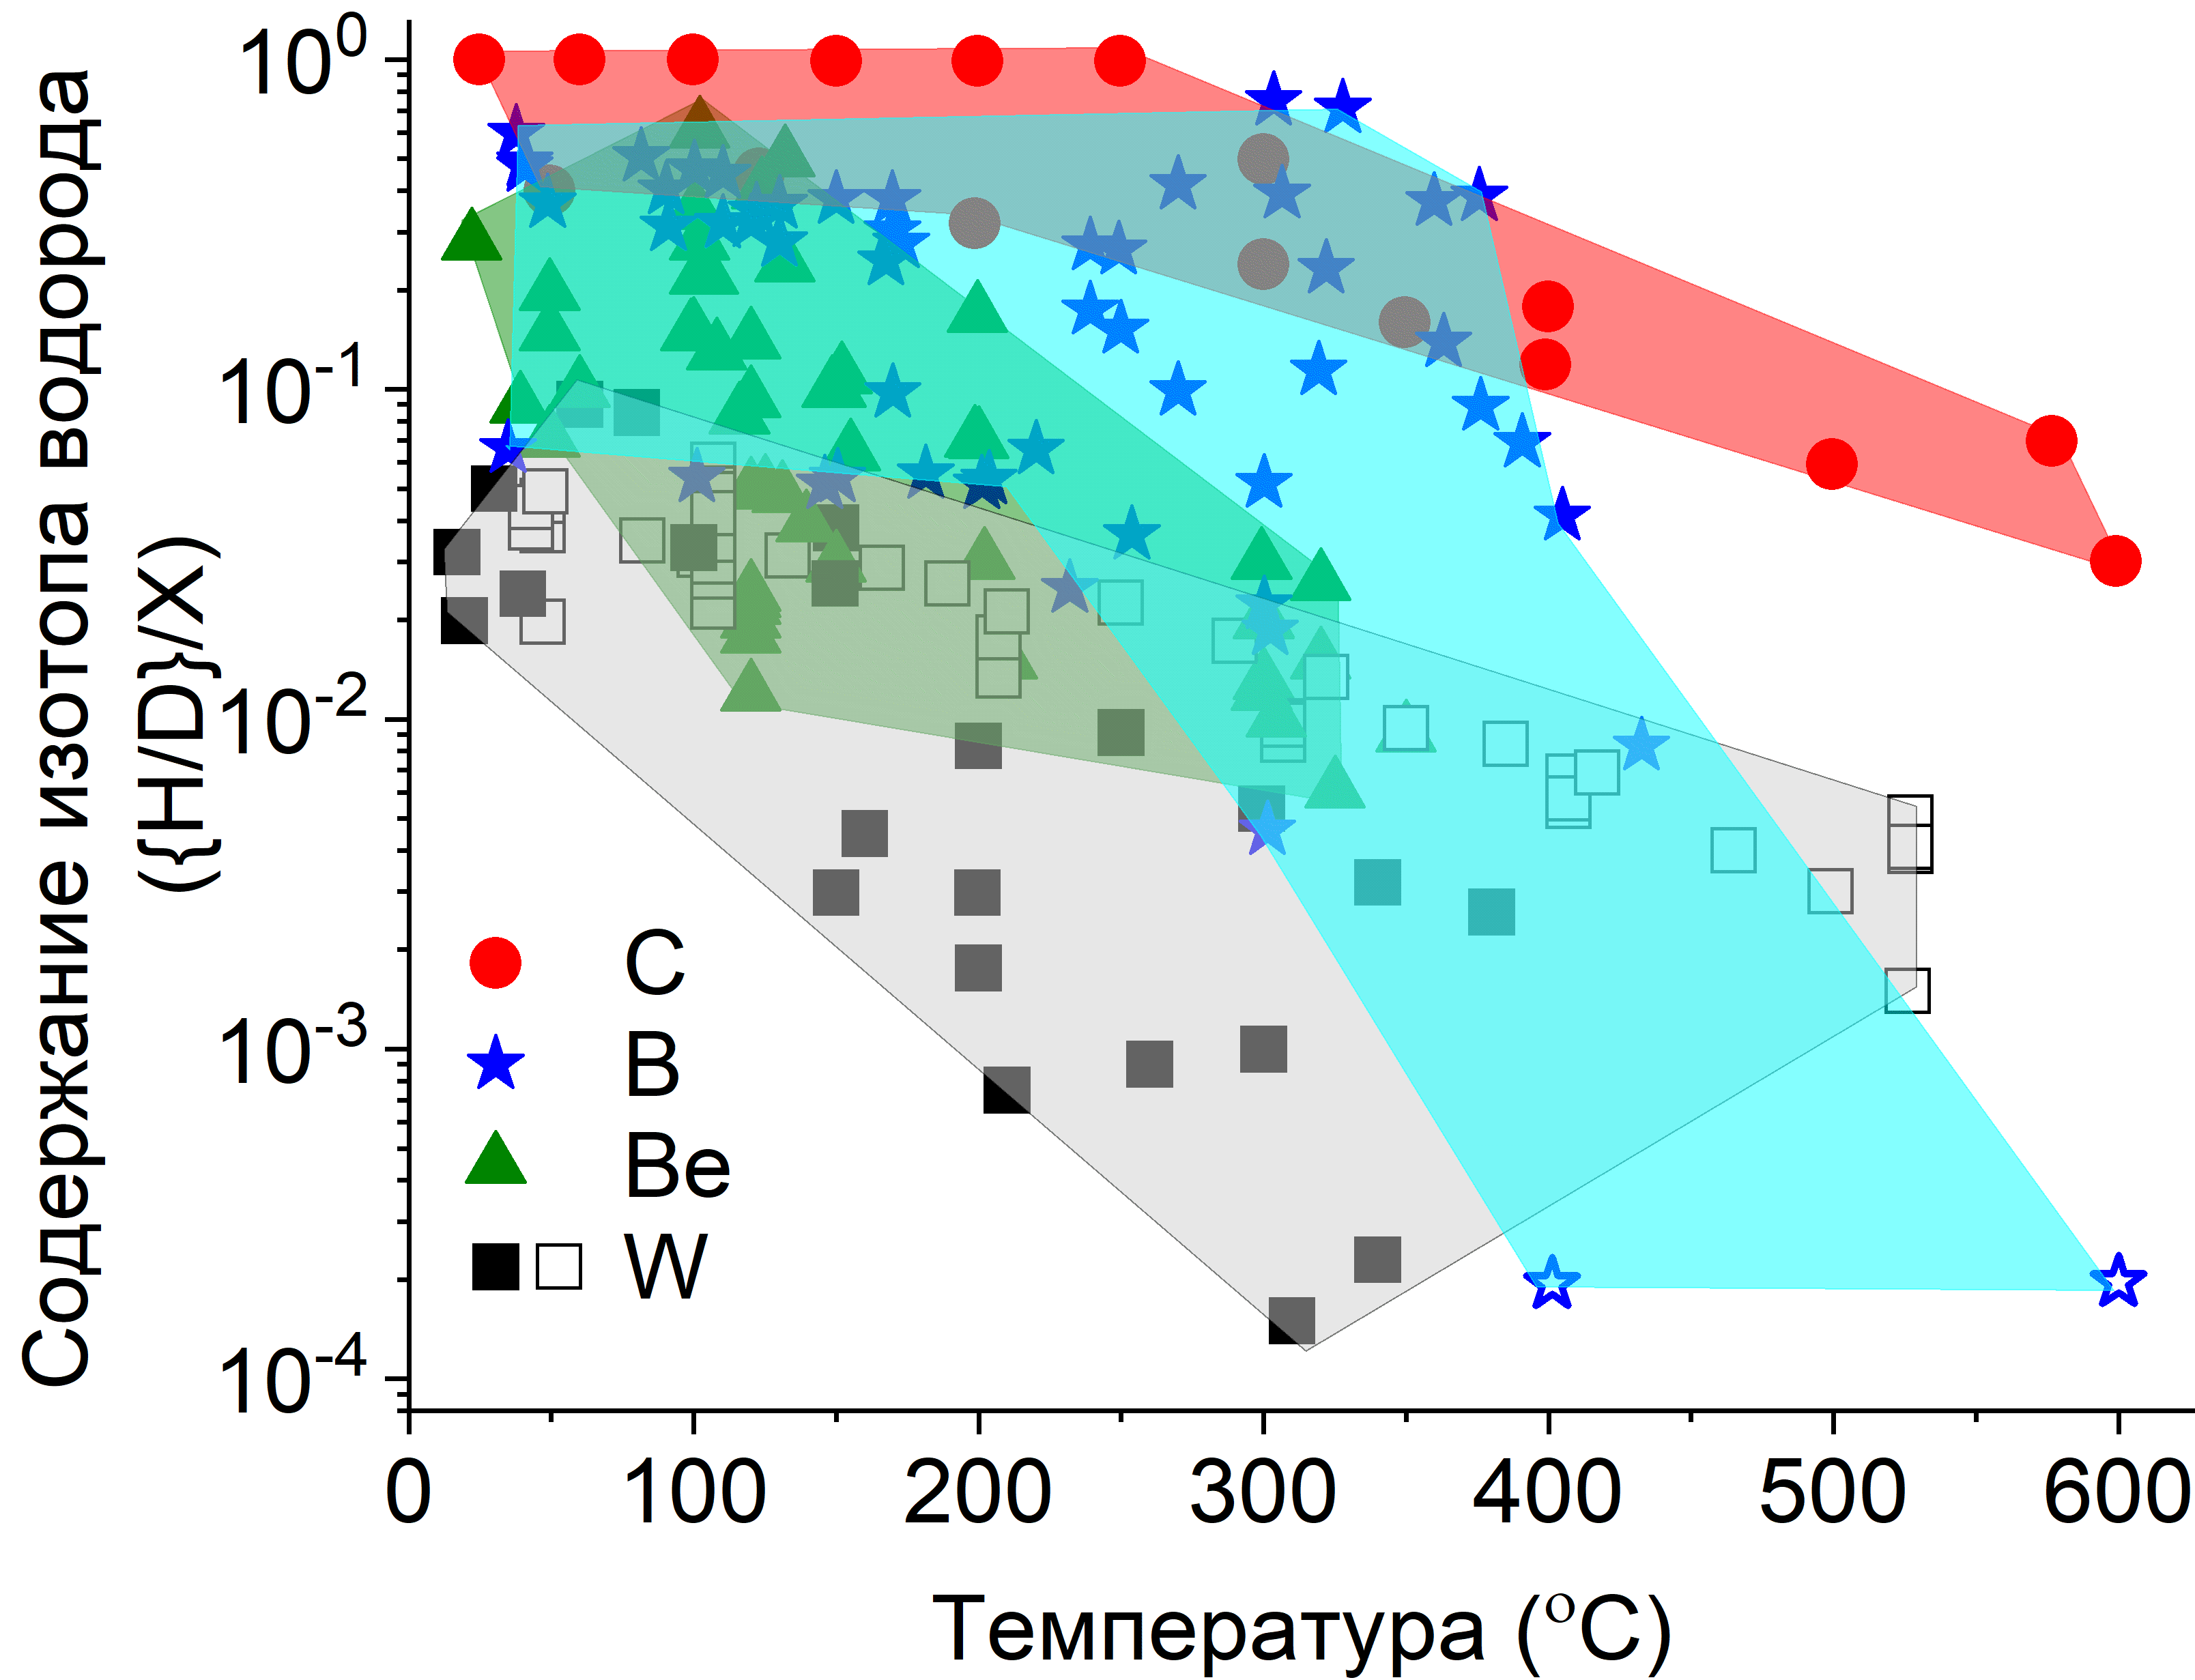
\includegraphics[scale=0.4]{codep_review.png}
    }
    \caption{Содержание изотопов водорода в зависимости от температуры совместного осаждения для пленок бора (голубая область), вольфрама (серая область), бериллия (зеленая область) и углерода (красная область)~\cite{Pitts2025}}\label{fig:ch1/codeposition_review}
\end{figure}
Примечательно, что содержание водорода оказывается систематически меньше в пленках вольфрама по сравнению с другими материалами. Помимо этого, скорость образования вольфрамовых пленок может быть меньше в ТЯУ из-за более высокого порога распыления. Однако недавний \textit{post-mortem} анализ образцов-свидетелей из токамака WEST указывает на образование переосажденных слоев с толщиной несколько микрометров~\cite{Bucalossi2024}.

\subsection{Взаимодействие изотопов водорода с вольфрамом}\label{subsec:ch1/sec3/subsec2}

Транспорт внедренных атомов водорода в вольфраме включает множество механизмов, которые можно разделить на несколько групп: диффузионные механизмы, взаимодействие с различными типами дефектов и поверхностные процессы. Качественное описание каждой из групп можно дать на основе одномерного представления пространственного распределения потенциальной энергии атомов водорода вблизи поверхности материала (см. рисунок~\cref{fig:ch1/potential_diagram_all}). Важно заметить, что в реальности ситуация оказывается гораздо сложнее, а распределение энергии водорода в материале с дефектами кристаллической решетки является трехмерным с совокупностью локальных экстремумов и седловых точек. Получение детальной информации о распределении потенциальной энергии возможно при помощи \textit{ab initio} методов, как теория функционала электронной плотности (DFT).

\nomenclature[A, 7]{DFT}{Теория функционала электронной плотности (Density functional theory)}

\begin{figure}[ht]
    \centerfloat{
        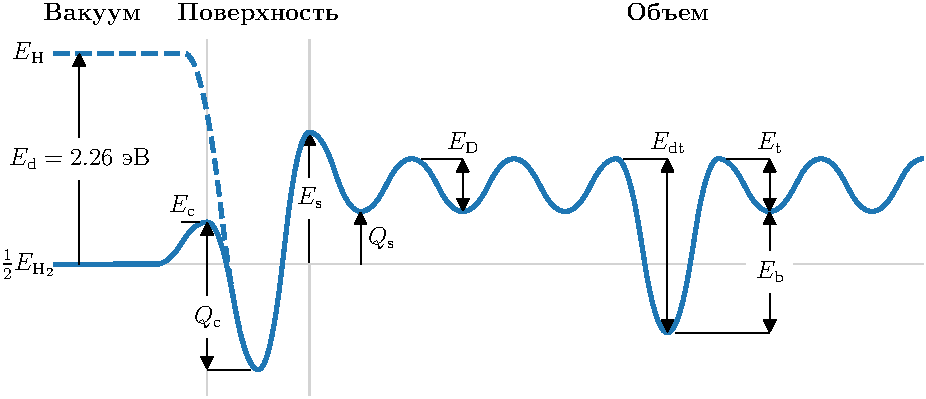
\includegraphics[scale=1]{potential_diagram_all.pdf}
    }
    \caption{Схематическая диаграмма потенциальной энергии водорода вблизи поверхности металла с положительной теплотой растворения. Уровни энергии отсчитываются от связанного состояния атома в молекуле водорода, расположенной далеко в вакууме}\label{fig:ch1/potential_diagram_all}
\end{figure}

\subsubsection{Диффузия}

Отталкивающий характер взаимодействия между атомами кристаллической решетки и водорода определяет предпочтительную оккупацию последним межузульных положений, являющимися локальными минимумами потенциальной энергии. Для вольфрама с объемно-центрированной кубической решеткой наиболее устойчивыми положениями являются тетраэдрическое и октаэдрическое, причем первое является более энергетически выгодным со значение теплоты растворения $Q_\mathrm{s}$ равным \SIrange{0.9}{1.0}{\electronvolt}~\cite{Heinola2010,Johnson2010,Fernandez2015,Zhou2024}. В процессе колебаний атомы водорода могут перескакивать между равновесными положениями, распространясь стохастически по объему материала. Направленный диффузионный поток атомов водорода $\mathbf{J}$ может быть обусловлен градиентами химического потенциала с вкладом $\mathbf{J}_c$ и температуры с вкладом $\mathbf{J}_T$~\cite{Longhurst1985, Krom1999, Martinez2021}:
\begin{equation}
    \mathbf{J}=\mathbf{J}_c+\mathbf{J}_T.
\end{equation}
В приближении малой концентрации растворенного водорода и отсутствия градиента напряжений в решетке вольфрама вклад от градиента химического потенциала можно редуцировать к влиянию градиента концентрации (закон Фика), определяющего поток $\mathbf{J}_{c}$:
\begin{equation}
    \mathbf{J}_{c} = -D \nabla \cm,
\end{equation}
где $D$ "--- коэффициент диффузии, \si{\meter\squared\per\second}; $\cm$ "--- концентрация атомов подвижного водорода, \si{\per\meter\cubed}. Диффузия, вызванная градиентом концентрации, является термоактивируемым процессом и в обычных условиях протекает быстрее с ростом температуры. Температурная зависимость коэффициента диффузии обычно описывается в соответствии с законом Аррениуса:
\begin{equation}
    D(T)=D_0 \exp\left( -\frac{E_\mathrm{D}}{k_\mathrm{B}T} \right),
\end{equation}
где $E_\mathrm{D}$ "--- энергия активации диффузии, \si{\electronvolt}; $k_\mathrm{B}=\SI{8.617e-5}{\electronvolt\per\kelvin}$ "--- постоянная Больцмана; $T$ "--- абсолютная температура, \si{\kelvin}.
\nomenclature[P, 02]{$Q_\mathrm{s}$}{Теплота растворения, \si{\electronvolt}}
\nomenclature[P, 03]{$J$}{Плотность потока атомов, \si{\per\meter\squared\per\second}}
\nomenclature[P, 04]{$J_{c}$}{Плотность потока атомов, индуцированного градиентом концентрации, \si{\per\meter\squared\per\second}}
\nomenclature[P, 05]{$J_{T}$}{Плотность потока атомов, индуцированного градиентом температуры, \si{\per\meter\squared\per\second}}
\nomenclature[P, 06]{$D$}{Коэффициент диффузии, \si{\meter\squared\per\second}}
\nomenclature[P, 07]{$\cm$}{Объемная концентрация подвижных атомов, \si{\per\meter\cubed}}
\nomenclature[P, 08]{$E_\mathrm{D}$}{Энергия активация диффузии, \si{\electronvolt}}
\nomenclature[P, 09]{$k_\mathrm{B}$}{Постоянная Больцмана, \si{\electronvolt\per\kelvin}}
\nomenclature[P, 10]{$T$}{Абсолютная температура, \si{\kelvin}}

Определение коэффициента диффузии проводилось как посредством экспериментов, так и путем моделирования. Параметры коэффициента диффузии, полученные Фраунфельдером ($D_0=\SI{4.1e-7}{\metre\squared\per\second}$, $E_\mathrm{D}=\SI{0.39}{\electronvolt}$, $T=\SIrange{1100}{2400}{K}$)~\cite{frauenfelder1969solution}, продолжительное время считались наиболее надежными. Последующие результаты моделирования методом DFT~\cite{Heinola2010,Johnson2010,Fernandez2015,Zhou2024} и недавние эксперименты~\cite{Holzner2020} указывают на большую подвижность атомов водорода в вольфраме с энергией активации диффузии в диапазоне \SIrange{0.2}{0.28}{\electronvolt}. Указанный диапазон согласуется с результатами Фраунфельдера при учете экспериментальных данных в высокотемпературной области, когда влиянием центров захвата на диффузию можно пренебречь~\cite{Heinola2010}. Тем не менее, значения коэффициента диффузии изотопов водорода сильно варьируются в литературе~\cite{remi_delaporte_mathurin_2024_13912922}, что значительно затрудняет проведение оценок накопления в материалах ОПЭ.

Облучение ОПЭ мощными тепловыми потоками неминуемо приведет к образованию температурных градиентов. Такая ситуация особо актуальна для конструкций элементов с активным водяным охлаждением, как диверторные моноблоки токамака ИТЭР. Градиент температур индуцирует поток термодиффузии $\mathbf{J}_T$ (эффект Соре):
\begin{equation}
    \mathbf{J}_{T} = -D\frac{\cm Q^*}{kT^2} \nabla T,
\end{equation}
направление которого определяется знаком теплоты переноса $Q^*$, \si{\electronvolt}.
\nomenclature[P, 11]{$Q^*$}{Теплота переноса, \si{\electronvolt}}

К сожалению, в настоящее время отсутствует общепринятое значение теплоты переноса водорода в вольфраме. Экспериментальные измерения показывают, что теплота переноса в металлах с положительной теплотой растворения отрицательна и незначительно растет с температурой~\cite{Longhurst1985}. Оценки величины для вольфрама методом молекулярной динамики~\cite{Martinez2021,Dasgupta2023} также подтверждают отрицательное значение, но определенная функциональная зависимость обратно пропорционально квадрату температуры:
\begin{equation}
    \label{eq:ch1/heat_transport}
    Q^*(T)=-0.0045 \kB T^2.
\end{equation}

\subsubsection{Центры захвата}

Дефекты в кристаллической решетке вольфрама, такие как вакансии, примеси, дислокации или пустоты, создают потенциальные энергетические ямы, более глубокие, чем междоузлия. Такие дефекты являются потенциальными <<ловушками>> для подвижных атомов водорода. Захваченные в <<ловушку>> атомы становится <<иммобильным>> и могут покинуть ее, если тепловой энергии достаточно для преодоления потенциального барьера $E_\mathrm{dt}$ [\si{\electronvolt}]. Упрощенный процесс захвата можно представить в следующем виде~\cite{Drexler2020}:
\begin{equation*}
    \underset{\text{дефект}}{[\quad]} + \underset{\text{междоузлие}}{(\mathrm{H})} \mathop{\rightleftharpoons}^{\nu_\mathrm{t}}_{\nu_\mathrm{dt}}  \underset{\text{дефект}}{[\mathrm{H}]} +  \underset{\text{междоузлие}}{(\quad)},
\end{equation*}
где \( \nu_\mathrm{t} \)"--- константа скорости захвата в дефект, \si{\metre\cubed\per\second}; \( \nu_\mathrm{dt}\)"--- константа скорости выхода из дефекта, \si{\per\second}. Обычно полагается, что скорость захвата определяется диффузией: \( E_\mathrm{t} \approx E_\mathrm{D} \). Это простейшее представление оказывается весьма удобным при построении численных моделей удержания водорода в материале. Описание процессов многочастичного захвата~\cite{Johnson2010,Fernandez2015} и изотопного обмена также возможно путем рассмотрения отдельных энергетических уровней атомов в дефекте и введения соответствующих скоростей перехода между ними~\cite{Schmid2014}.

\nomenclature[P, 12]{\( \nu_\mathrm{t} \)}{Константа скорости захвата атомов в дефекты, \si{\metre\cubed\per\second}}
\nomenclature[P, 13]{\( \nu_\mathrm{dt} \)}{Константа скорость выхода атомов из дефектов, \si{\per\second}}
\nomenclature[P, 14]{\( E_\mathrm{t} \)}{Энергия активация захвата в дефект, \si{\electronvolt}}
\nomenclature[P, 15]{\( E_\mathrm{dt} \)}{Энергия активации выхода из дефекта, \si{\electronvolt}}

Дефекты в материале можно классифицировать на два типа. Первый тип, часто называемый собственными (естественными) дефектами, является свойственным материалу: примеси в сплавах, границы зерен поликристаллических металлов, элементарные дефекты малой концентрации, образованные в ходе процесса производства. Второй тип, внешние (индуцированные) дефекты, возникают в результате внешних воздействий на материал, включая повреждения от бомбардировки частицами (ионами или нейтронами) или механического напряжения, и могут развиваться во времени и пространстве. Получение информации о параметрах центров захвата возможно экспериментально или путем моделирования. Атомистическое моделирование методом DFT позволяет рассчитать энергию связи атома с дефектом \( E_\mathrm{b} \), когда рамках экспериментов наиболее надежно определяют барьер выхода из ловушек \( E_\mathrm{dt}=E_\mathrm{b} + E_\mathrm{t} \). Широко распространенным методом определения энергетического барьера выхода дефектов является термодесорбционная спектроскопия (ТДС). Дополнительную информацию о свойствах и пространственном распределении центров захвата позволяют получить ионно-пучковые методы анализа, например метод ядерных реакций (МЯР). 

\nomenclature[A, 8]{ТДС}{Термодесорбционная спектроскопия}
\nomenclature[A, 9]{МЯР}{Метод ядерных реакций}

Энергия связи атома водорода с дефектами зависит от их типа. Детальная информация об энергии связи приведена в исчерпывающих обзорах~\cite{Ogorodnikova2015,Li2020,Persianova2024}. Отметим наиболее распространенные типы атомистических дефектов в вольфраме. Наименьшей энергией связи (\SIrange{0.65}{1.25}{\electronvolt}) с атомами водорода характеризуются дислокации. Больная сильная связь наблюдается между атомами растворенного водорода и вакансиями кристаллической решетки вольфрама с энергией связи \SIrange{1.05}{1.55}{\electronvolt}. Энергия связи увеличивается с ростом числа вакансий, агломерированных в вакансионный кластер, и спадает с числом атомов водорода, захваченных в них. Наибольшая энергия связи соответствует полостям в вольфраме с диапазоном значений от \num{2.05} до \SI{2.45}{\electronvolt}. Из приведенной краткой характеристики можно заметить, что литературные данные для различных дефектами пересекаются, что усложняет определение типа дефекта при экспериментальном анализе. Помимо этого, в ходе ионного и нейтронного облучения образуются каскады смещений, формируя сложные комплексы дефектов, а достижение определенной дозы накопленных изотопов водорода может инициировать образование микроскопических дефектов, как блистеры~\cite{Wang2001}. 

\subsubsection{Поверхностные процессы}

Поверхностные процессы играют ключевую роль во множестве областей. Так, стандартным методом исследования водородного охрупчивания материалов является их насыщение водородом из газовой фазы~\cite{Briant2002,Louthan2008}. Кроме того, известно, что поверхностные процессы играют фундаментальную роль в образовании молекулярного водорода в межзвездной среде~\cite{Katz1999, Perets2005, Hama2013}. При температурах, близких к нулю, типичных для плотных межзвездных облаков, обилие молекулярного водорода в основном объясняется эффективной рекомбинационной десорбцией на поверхности пыли, протекающей более интенсивно по сравнению с другими процессами в газовой фазе. Учет влияния поверхностных процессов также требовался для интерпретации некоторых результатов ТДС измерений~\cite{Hodille2017, Matveev2018}.

Для эндотермических металлов свободная поверхность является стоком атомов водорода из-за более низкого уровня потенциальной энергии по сравнению с растворенным состоянием (см. рисунок~\cref{fig:ch1/potential_diagram_all}). В процессе тепловой миграции внедренные атомы могут переходить в адсорбированное состояние из приповерхностной области при преодоление энергетического барьера \( E_\mathrm{bs}=E_\mathrm{s}-Q_\mathrm{s} \), где \( E_\mathrm{s} \) есть энергия активации растворения, \si{\electronvolt}. Таким образом, адсорбированные атомы образуют отдельную фракцию, характеризующуюся поверхностной концентрацией \( \csurf \), \si{\per\meter\squared}. Величина энергии активации растворения может варьироваться в зависимости от наличия примесей в приповерхностной области, но в расчетах для <<чистой>> поверхности обычно полагается \( E_\mathrm{s} \approx E_\mathrm{D} + Q_\mathrm{s} \), что также определяет барьер перехода в адсорбированное состояние \(  E_\mathrm{bs} \approx E_\mathrm{D} \). Энергия связи адсорбированного атома с поверхностью определяется глубиной потенциальной ямы (теплотой) хемосорбции \( Q_\mathrm{c} \), \si{\electronvolt}. Наряду с выходом на поверхность возможен обратный процесс абсорбции, если энергии атома достаточно для преодоления барьера \( E_\mathrm{sb} = E_\mathrm{s} - Q_\mathrm{c} \). Переходам между адсорбированным и растворенным состояниями можно охарактеризовать аналогично процессам захвата и выхода из ловушек, введя константы скорости выхода на поверхность (\( \nubs \), \si{\meter\per\second}) и обратной абсорбции (\( \nusb \), \si{\per\second}), определяющие соответствующие потоки частиц.

Другой группой процессов, влияющих на эволюцию поверхностной концентрации, являются химическая адсорбция\footnote{Далее в работе термины <<химическая адсорбция>>, <<хемосорбция>> и <<адсорбция>> будут использованы как взаимозаменяемые, когда физическая адсорбция рассмотрена не будет.} и десорбция. На поверхности возможно протекание различных типов реакций с участием одного или нескольких адсорбированных атомов водорода (см. рисунок~\cref{fig:ch1/surface_processes}): диссоциативная адсорбция молекул водорода, рекомбинация двух адсорбированных атомов (рекомбинация Ленгмюра-Хиншельвуда), рекомбинация медленного атома/иона, приходящего на поверхность, и адсорбированного атома (рекомбинация Или-Ридила\footnote{В литературе данный тип десорбции обычно называется механизмом Или-Ридила, однако в некоторых источниках~\cite{Prins2018} отмечается, что в оригинальных работах Д. Или и Э. Ридила дается описание взаимодействия хемосорбированного и физиосорбированного атомов, когда для рассматриваемого процесса корректным названием будет <<механизм Ленгмюра-Ридила>>. В рамках данной работы будет использован термин <<механизм Или-Ридила>> из-за его большей распространенности.}), рекомбинация надтеплового (<<hot atom>>) атома с адсорбированным, распыление при облучении ионами, а также десорбция/адсорбция атомов. 

\begin{figure}[ht]
    \centerfloat{
        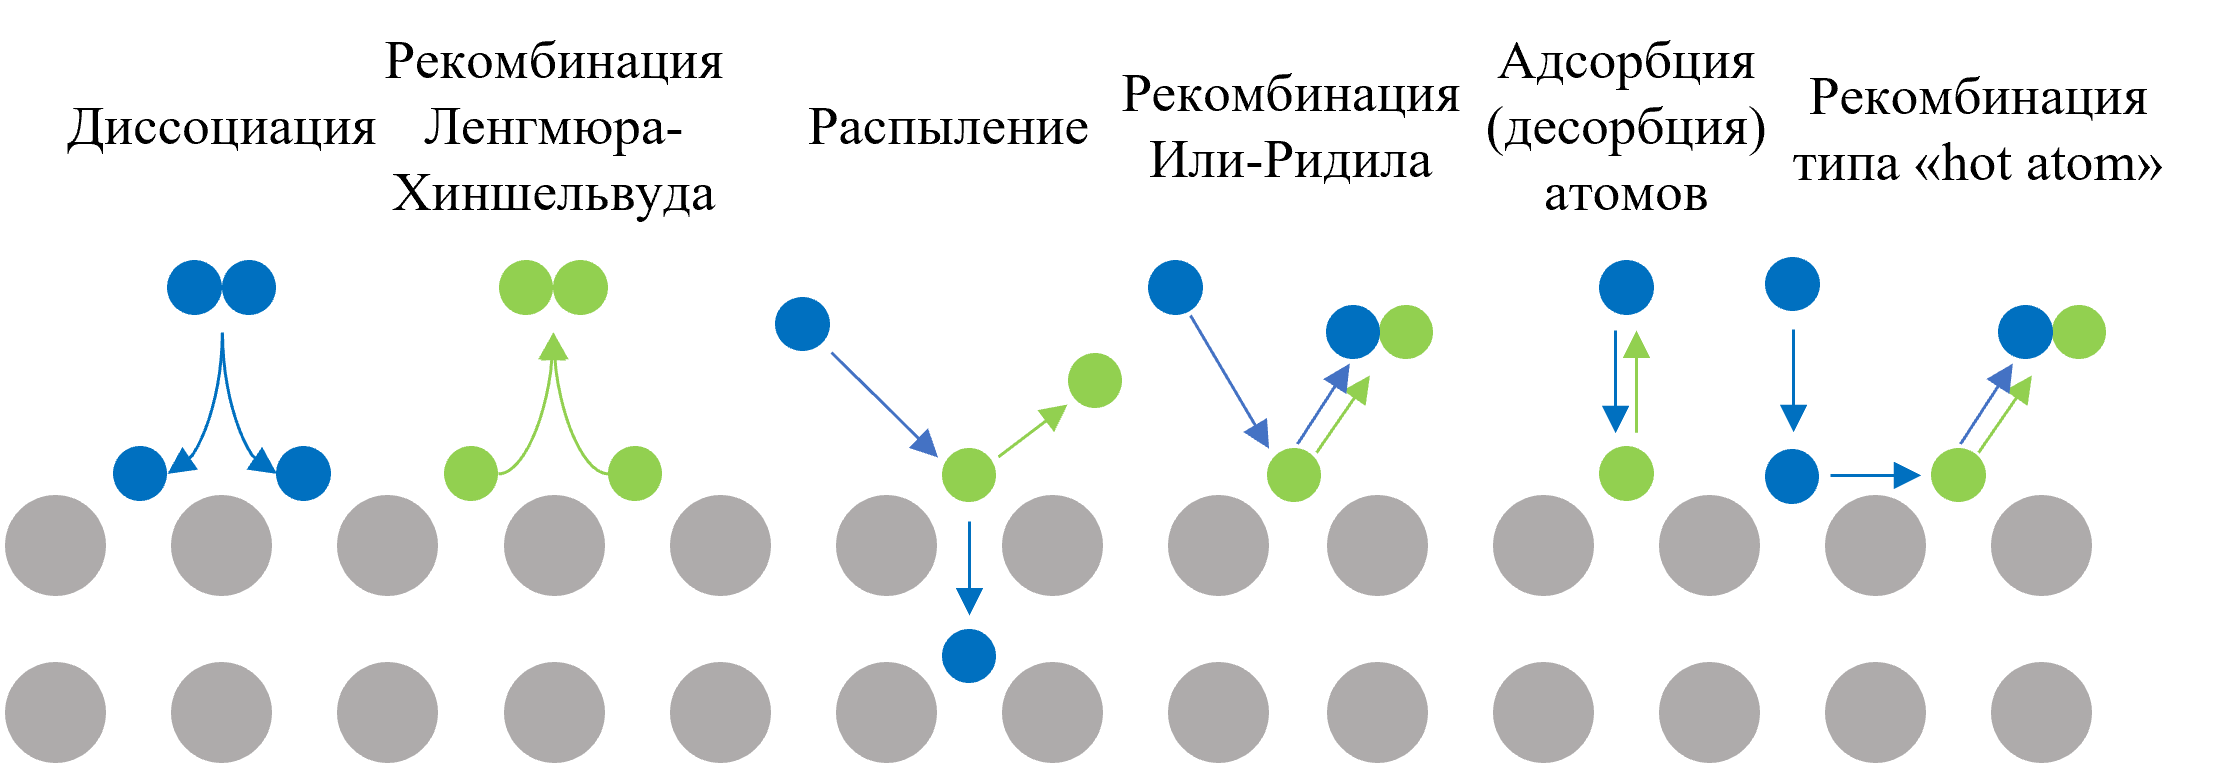
\includegraphics[scale=1]{surface_processes.png}
    }
    \caption{Схематическое представление некоторых процессы, происходящих на поверхности металла. Синие круги представляют падающие частицы (атомы или молекулы) из приповерхностной среды, зеленые круги соответствуют изначально адсорбированным атомам, серые "--- атомам материала поверхности}\label{fig:ch1/surface_processes}
\end{figure}

Плотность потока десорбированных частиц \( J_{\mathrm{des}} \) в \si{\per\meter\squared\per\second} можно описать в зависимости от порядка десорбции \( n \):
\begin{equation}
    \label{eq:ch1/des_flux}
    J_{\mathrm{des}} = n \nu_\mathrm{des} \csurf^n,
\end{equation}
где \( \nudes=\nu_{\mathrm{des},0} \exp \left( -E_\mathrm{des} / \kBT \right) \) "--- константа скорости десорбции, \si{\meter^{2(n-1)} \per \second}; \( E_\mathrm{des} \) "--- энергия активации десорбции, \si{\electronvolt}. Упомянутые ранее механизмы десорбции соответствуют $n=1$ (десорбция атомов, механизм Или-Ридила, т.д.) и $n=2$ (механизм Ленгмюра-Хиншельвуда, реакция типа <<hot atom>>). Каналы десорбции молекул по схеме Ленгмюра-Хиншельвуда и атомов являются термически активируемыми. Также можно отметить, что в ряде работ~\cite{Baskes1980, Richards1988, Pisarev1997} рассматривались каналы десорбции с участием одного или двух атомов из приповерхностной области. \fixme{Рассмотрение данных механизмов проводится в главе 3.}

Вероятность десорбции по каналу Ленгмюра-Хиншельвуда глубиной потенциальной ямы (теплотой) хемосорбции и энергией активации хемосорбции \( E_\mathrm{c} \), \si{\electronvolt}. Согласно экспериментальным оценкам~\cite{Tamm1969,Tamm1971,Markelj2013} и моделированию методом DFT~\cite{Piazza2018,Ajmalghan2019,Ferro2023}, барьер десорбции молекул лежит в диапазоне \SIrange{0.25}{1.1}{\electronvolt} в зависимости от состояния поверхности и концентрации адсорбированного водорода. Обратный механизм протекает при диссоциации молекул у поверхности с преодоление барьера \( E_\mathrm{diss}=2E_\mathrm{c} \) и последующей адсорбцией двух атомов. В случае чистой поверхности адсорбция частиц происходить безактивационно (\( E_\mathrm{c} \approx 0 \))~\cite{Piazza2018,Ajmalghan2019,Ferro2023}. Десорбция атомов требует преодоления гораздо большего барьера (\( E_\mathrm{des}=E_\mathrm{d}-Q_\mathrm{c} \)), что возможно при высоких температурах поверхности ввиду относительно большой разницы между энергетическими уровнями (\(E_\mathrm{d}=\SI{2.26}{\electronvolt}\)) атома водорода в свободном и связанном в молекуле состоянии.

При локальном равновесии вблизи поверхности и пределе малой доли водорода в металле концентрации на поверхности и в приповерхностной области связаны следующим соотношением~\cite{Pick1985}:
\begin{equation}
    \label{eq:ch1/bs_equilibrium}
    \csurf = \cm \frac{\nubs}{\nusb}.
\end{equation}
Подстановка данного выражения в уравнение~\eqref{eq:ch1/des_flux} приводит к:
\begin{equation}
    J_{\mathrm{des}} = n \nu_\mathrm{des} \left( \frac{\nubs}{\nusb} \right)^n \cm^n=K_\mathrm{r} \cm^n,
\end{equation}
где \( K_\mathrm{r} \) "--- коэффициент рекомбинации на поверхности, \si{\meter^{3n-2}}. Применение коэффициента рекомбинации оправдано, когда процессы в объеме протекают гораздо медленнее поверхностных. Данный подход позволяет упростить задачу транспорта изотопов водорода в материалах, что удобно при проведении численного моделирования. Наиболее распространенными в литературе коэффициентами рекомбинации водорода на поверхности вольфрама (в \si{\meter^4\per\second}) являются аналитический коэффициент рекомбинации Пика-Сонненберга~\cite{Pick1985}:
\begin{equation}
    \label{eq:ch1/Kr_PS}
    K_\mathrm{r}(T) = \frac{\num{3e-25}}{\sqrt{T}} \exp \left( \frac{Q_\mathrm{s}-E_\mathrm{c}}{\kBT} \right),
\end{equation}
и эмпирический коэффициент Андерла~\cite{Anderl1992}
\begin{equation}
    K_\mathrm{r}(T) = \num{3.2e-15} \exp \left( -\frac{\SI{1.16}{[\electronvolt]}}{\kBT} \right).
\end{equation}
Приведенные выражения имеют совершенно разную функциональную зависимость от температуры, причем показатель экспоненты в выражении~\cref{eq:ch1/Kr_PS} становится отрицательным исключительно при наличии большого барьера хемосорбции на поверхности. В работе~\cite{Ogorodnikova2019} продемонстрировано, что применение коэффициента рекомбинации Андерла приводит к существенному завышению проникающего потока, что вызывает несоответствие с экспериментальными данными.

Помимо применения коэффициентов рекомбинации, распространенной аппроксимацией процессов на поверхности является приближение бесконечно быстрой рекомбинации. Качественное представление можно получить, рассмотрев точечный источник имплантированных атомов с плотностью потока \( \Gamma \). При достижении равновесия поток атомов, диффундирующих вглубь материала становится мал, а поток десорбированных частиц уравновешивается потоком имплантируемых. Учитывая равенство~\cref{eq:ch1/bs_equilibrium} при локальном равновесии и полагая, что с поверхности десорбируются двуатомные молекулы, можно получить выражение для максимальной концентрации атомов растворенного водорода вблизи поверхности: 
\begin{equation}
    \cm = \sqrt{\frac{\Gamma}{K_\mathrm{r}}},
\end{equation}
которое в пределе бесконечно большой скорости рекомбинации упрощается до вида: \( \cm=0 \).

Еще одной важной величиной является растворимость водорода в вольфраме. Выражение для растворимости можно получить, рассмотрев поверхность, находящуюся в равновесии с газом при давлении \( P \) (в \si{\pascal}). Поток частиц (\( J_\mathrm{ads} \), \si{\per\meter\squared\per\second}), сорбирующихся на поверхность из газовой фазы, имеет следующее представление: 
\begin{equation}
    J_\mathrm{ads} = n \nu_{\mathrm{ads}} \Gamma,
\end{equation}
где \( \nu_{\mathrm{ads}} \) "--- константа скорости адсорбции молекул из газовой фазы, \si{\per\meter\squared\per\second\per\pascal}. При локальном равновесии потоки адсорбирующихся и десорбирующихся частиц равны. Учитывая выражения~\eqref{eq:ch1/des_flux} и \eqref{eq:ch1/bs_equilibrium}, можно получить:
\begin{equation}
    \cm = \sqrt[n]{\frac{\nu_\mathrm{ads}}{\nu_\mathrm{des}}}\sqrt[n]{P}.
\end{equation}
Для двуатомных молекул водорода выражение упрощается до вида: \( \cm = K_\mathrm{s} \sqrt{P} \), описывающее закон растворения Сивертса с константой \( K_\mathrm{s}=K_{\mathrm{s},0} \exp \left( -Q_\mathrm{s}/\kBT \right) \). Наиболее распространенное значение растворимости (в \( \si{\per\meter\cubed}\cdot\si{\pascal}^{-0.5} \)) было измерено Фраунфельдером~\cite{frauenfelder1969solution}:
\begin{equation}
    K_\mathrm{s}(T) = \num{8.88e23} \exp \left( -\frac{\SI{1.04}{[\electronvolt]}}{\kBT} \right).
\end{equation}

\nomenclature[P, 16]{\( E_\mathrm{bs} \)}{Энергетический барьер перехода из растворенного состояния в адсорбированное, \si{\electronvolt}}
\nomenclature[P, 17]{\( E_\mathrm{sb} \)}{Энергетический барьер перехода из адсорбированного состояния в растворенное, \si{\electronvolt}}
\nomenclature[P, 18]{\( E_\mathrm{s} \)}{Энергия активации растворения, \si{\electronvolt}}
\nomenclature[P, 19]{\( Q_\mathrm{C} \)}{Теплота хемосорбции, \si{\electronvolt}}
\nomenclature[P, 20]{\( \nubs \)}{Константа скорости перехода из растворенного состояния в адсорбированное, \si{\meter\per\second}}
\nomenclature[P, 21]{\( \nusb \)}{Константа скорости перехода из адсорбированного состояния в растворенное, \si{\per\second}}
\nomenclature[P, 22]{\( \csurf \)}{Поверхностная концентрация адсорбированных атомов, \si{\per\meter\squared}}
\nomenclature[P, 23]{\( J_\mathrm{des} \)}{Поток десорбированных атомов, \si{\per\meter\squared\per\second}}
\nomenclature[P, 24]{\( J_\mathrm{ads} \)}{Поток адсорбирующихся (хемосорбирующихся) атомов, \si{\per\meter\squared\per\second}}
\nomenclature[P, 25]{\( E_\mathrm{des} \)}{Энергетический барьер десорбции, \si{\electronvolt}}
\nomenclature[P, 26]{\( K_\mathrm{r} \)}{Коэффициент рекомбинации, \si{\meter^4\per\second}}
\nomenclature[P, 27]{\( K_\mathrm{s} \)}{Константа растворимость, \si{\per\meter\cubed\per\pascal^{0.5}}}
\nomenclature[P, 28]{\( P \)}{Давление, \si{\pascal}}
\nomenclature[P, 29]{\( E_\mathrm{diss} \)}{Энергия активации диссоциации молекулы с последующей хемосорбцией двух атомов, \si{\electronvolt}}
\nomenclature[P, 30]{\( E_\mathrm{d} \)}{Энергия диссоциации молекулы водорода, \si{\electronvolt}}

\subsection{Накопление при стационарном плазменном облучении}\label{sec:ch1/sec3/subsec3}

Краткий обзор основных каналов механизмов взаимодействия указывает на комплексность процессов, определяющих захват изотопов водорода в вольфраме. Динамика накопления водорода в вольфраме была и является предметом интенсивных научных исследований. Условия облучения и подготовка образцов определяют долю накопленного дейтерия в вольфраме. На рисунке~\cref{fig:ch1/retention_fluence} приведены результаты ряда экспериментов, проведенных при ионном и плазменном облучении. Наблюдается широкий разброс в интегральном накоплении при различных условиях эксперимента, однако скорость накопления в них хорошо согласуется с корневой зависимостью от дозы облучения, что соответствует механизму накопления, определяемому диффузией.  

\begin{figure}[ht]
    \centerfloat{
        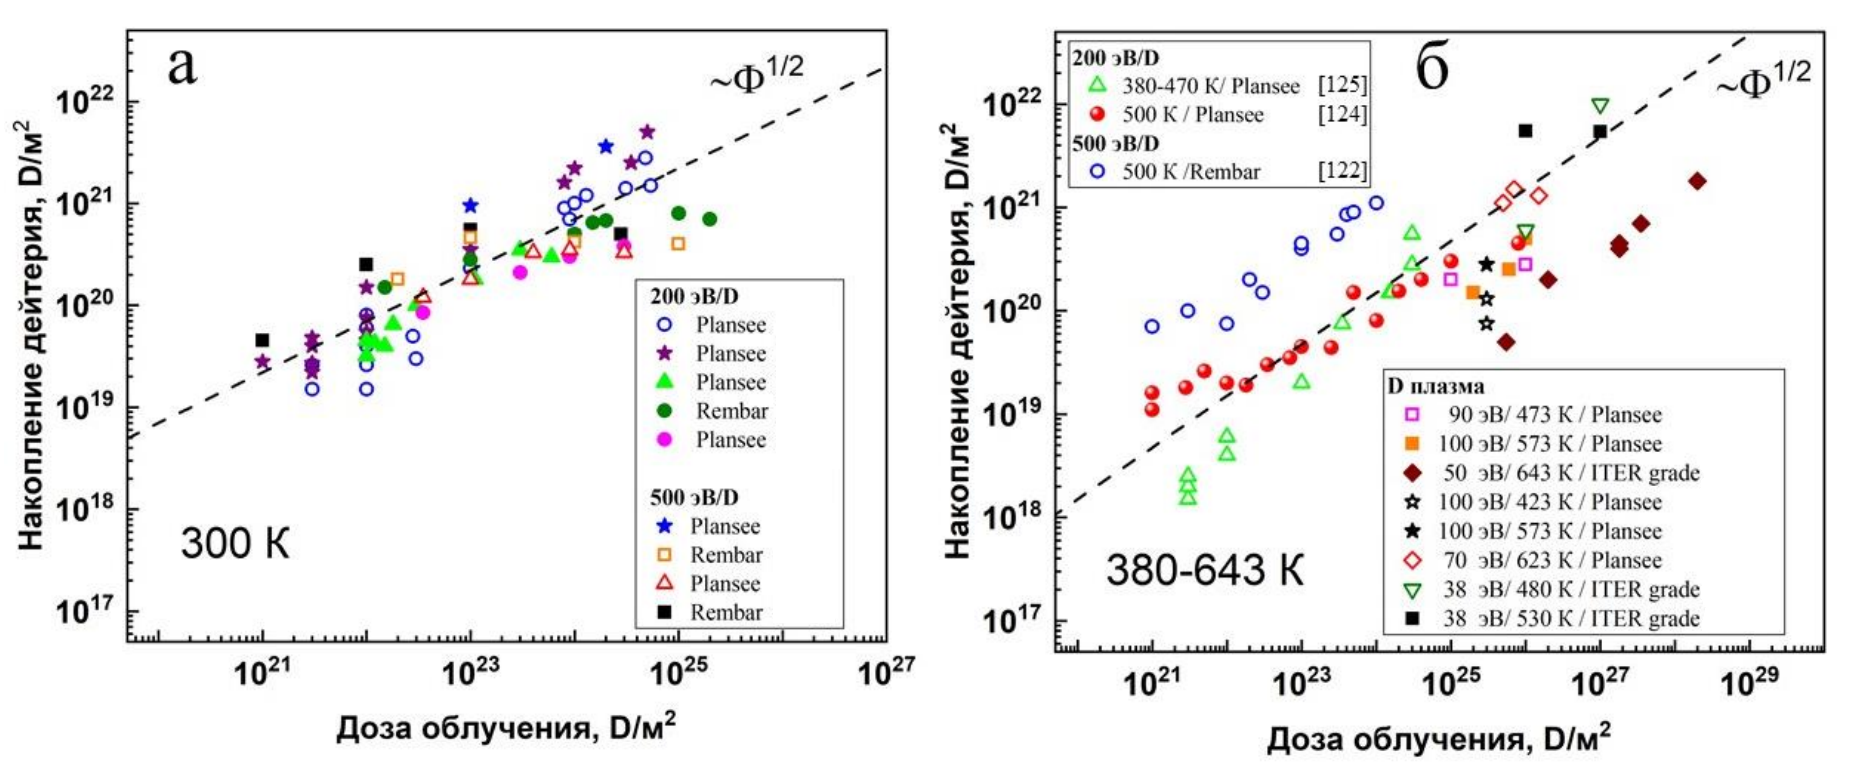
\includegraphics[scale=0.35]{retention_fluence.png}
    }
    \caption{Зависимость интегрального содержания дейтерия в поликристаллическом вольфраме от дозы облучения: а) ионным пучком при комнатной температуре; б) ионным пучком и плазмой при температуре в диапазоне \SIrange{380}{643}{\kelvin}~\cite{HarutunyanThesis}}\label{fig:ch1/retention_fluence}
\end{figure}

Содержание водорода в вольфраме во много определяется динамикой развития центров захвата. Облучение поверхности до больших доз частиц может приводить к образованию слоя перенасыщения в области внедрения (\( \sim \SI{10}{\nano\meter} \)), когда концентрация растворенного водорода превышает предел растворимости. Предполагается, что развитие процесса происходит за счет индуцирования напряжений в приповерхностной области, облегчающих создание новых центров захвата для внедряемого водорода~\cite{Nishijima2023}. Дальнейшее развитие поверхности при ионном облучении может сопровождаться появлением блистеров. Цикличные процессы образования и разрушения блистеров влияют на динамику удержания в приповерхностной области, а также препятствует распространению водорода вглубь материала~\cite{Bauer2017}.  

Несмотря на возможное достижение высокой доли (\( \approx \SI{10}{\text{ат.}\percent} \)) захваченного водорода, глобальное удержание топлива не должно сильно зависеть от этих приповерхностных механизмов ввиду малой толщины затрагиваемой области. Во время работы реактора образование дефектов будет происходит по всему объему ОПЭ в результате непрерывной бомбардировки нейтронами высокой энергии. В настоящее время нет ресурсов для исследования эффекта термоядерных нейтронов на накопление изотопов водорода в материалах. Распространенным подходом является использование ионов тяжелых элементов с энергией порядка нескольких мегаэлектронвольт для имитации повреждений, создаваемых нейтронным облучением в приповерхностной области. Результаты некоторых экспериментов по накоплению дейтерия после предварительного облучения МэВ-ными ионами приведены на рисунке~\cref{fig:ch1/retention_dpa}. Индуцированное число смещений на атом в ИТЭР оценивается на уровне \num{0.6} и \num{1.0} для дивертора и первой стенки, соответственно. Экстраполяция экспериментальных данных на указанный диапазон показывает, что концентрация захваченных изотопов водорода в вольфраме может достигать \( \sim \SI{1}{\text{ат.}\percent} \). 

\begin{figure}[ht]
    \centerfloat{
        \hfill
        \subcaptionbox[List-of-Figures entry]{\label{fig:ch1/retention_dpa}}{%
            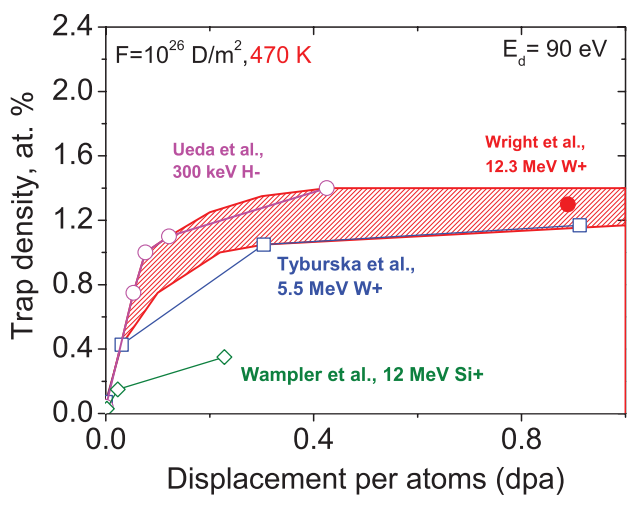
\includegraphics[width=0.49\linewidth]{retention_dpa.png}}
        \hfill
        \subcaptionbox{\label{fig:ch1/retention_HeTemperature}}{%
            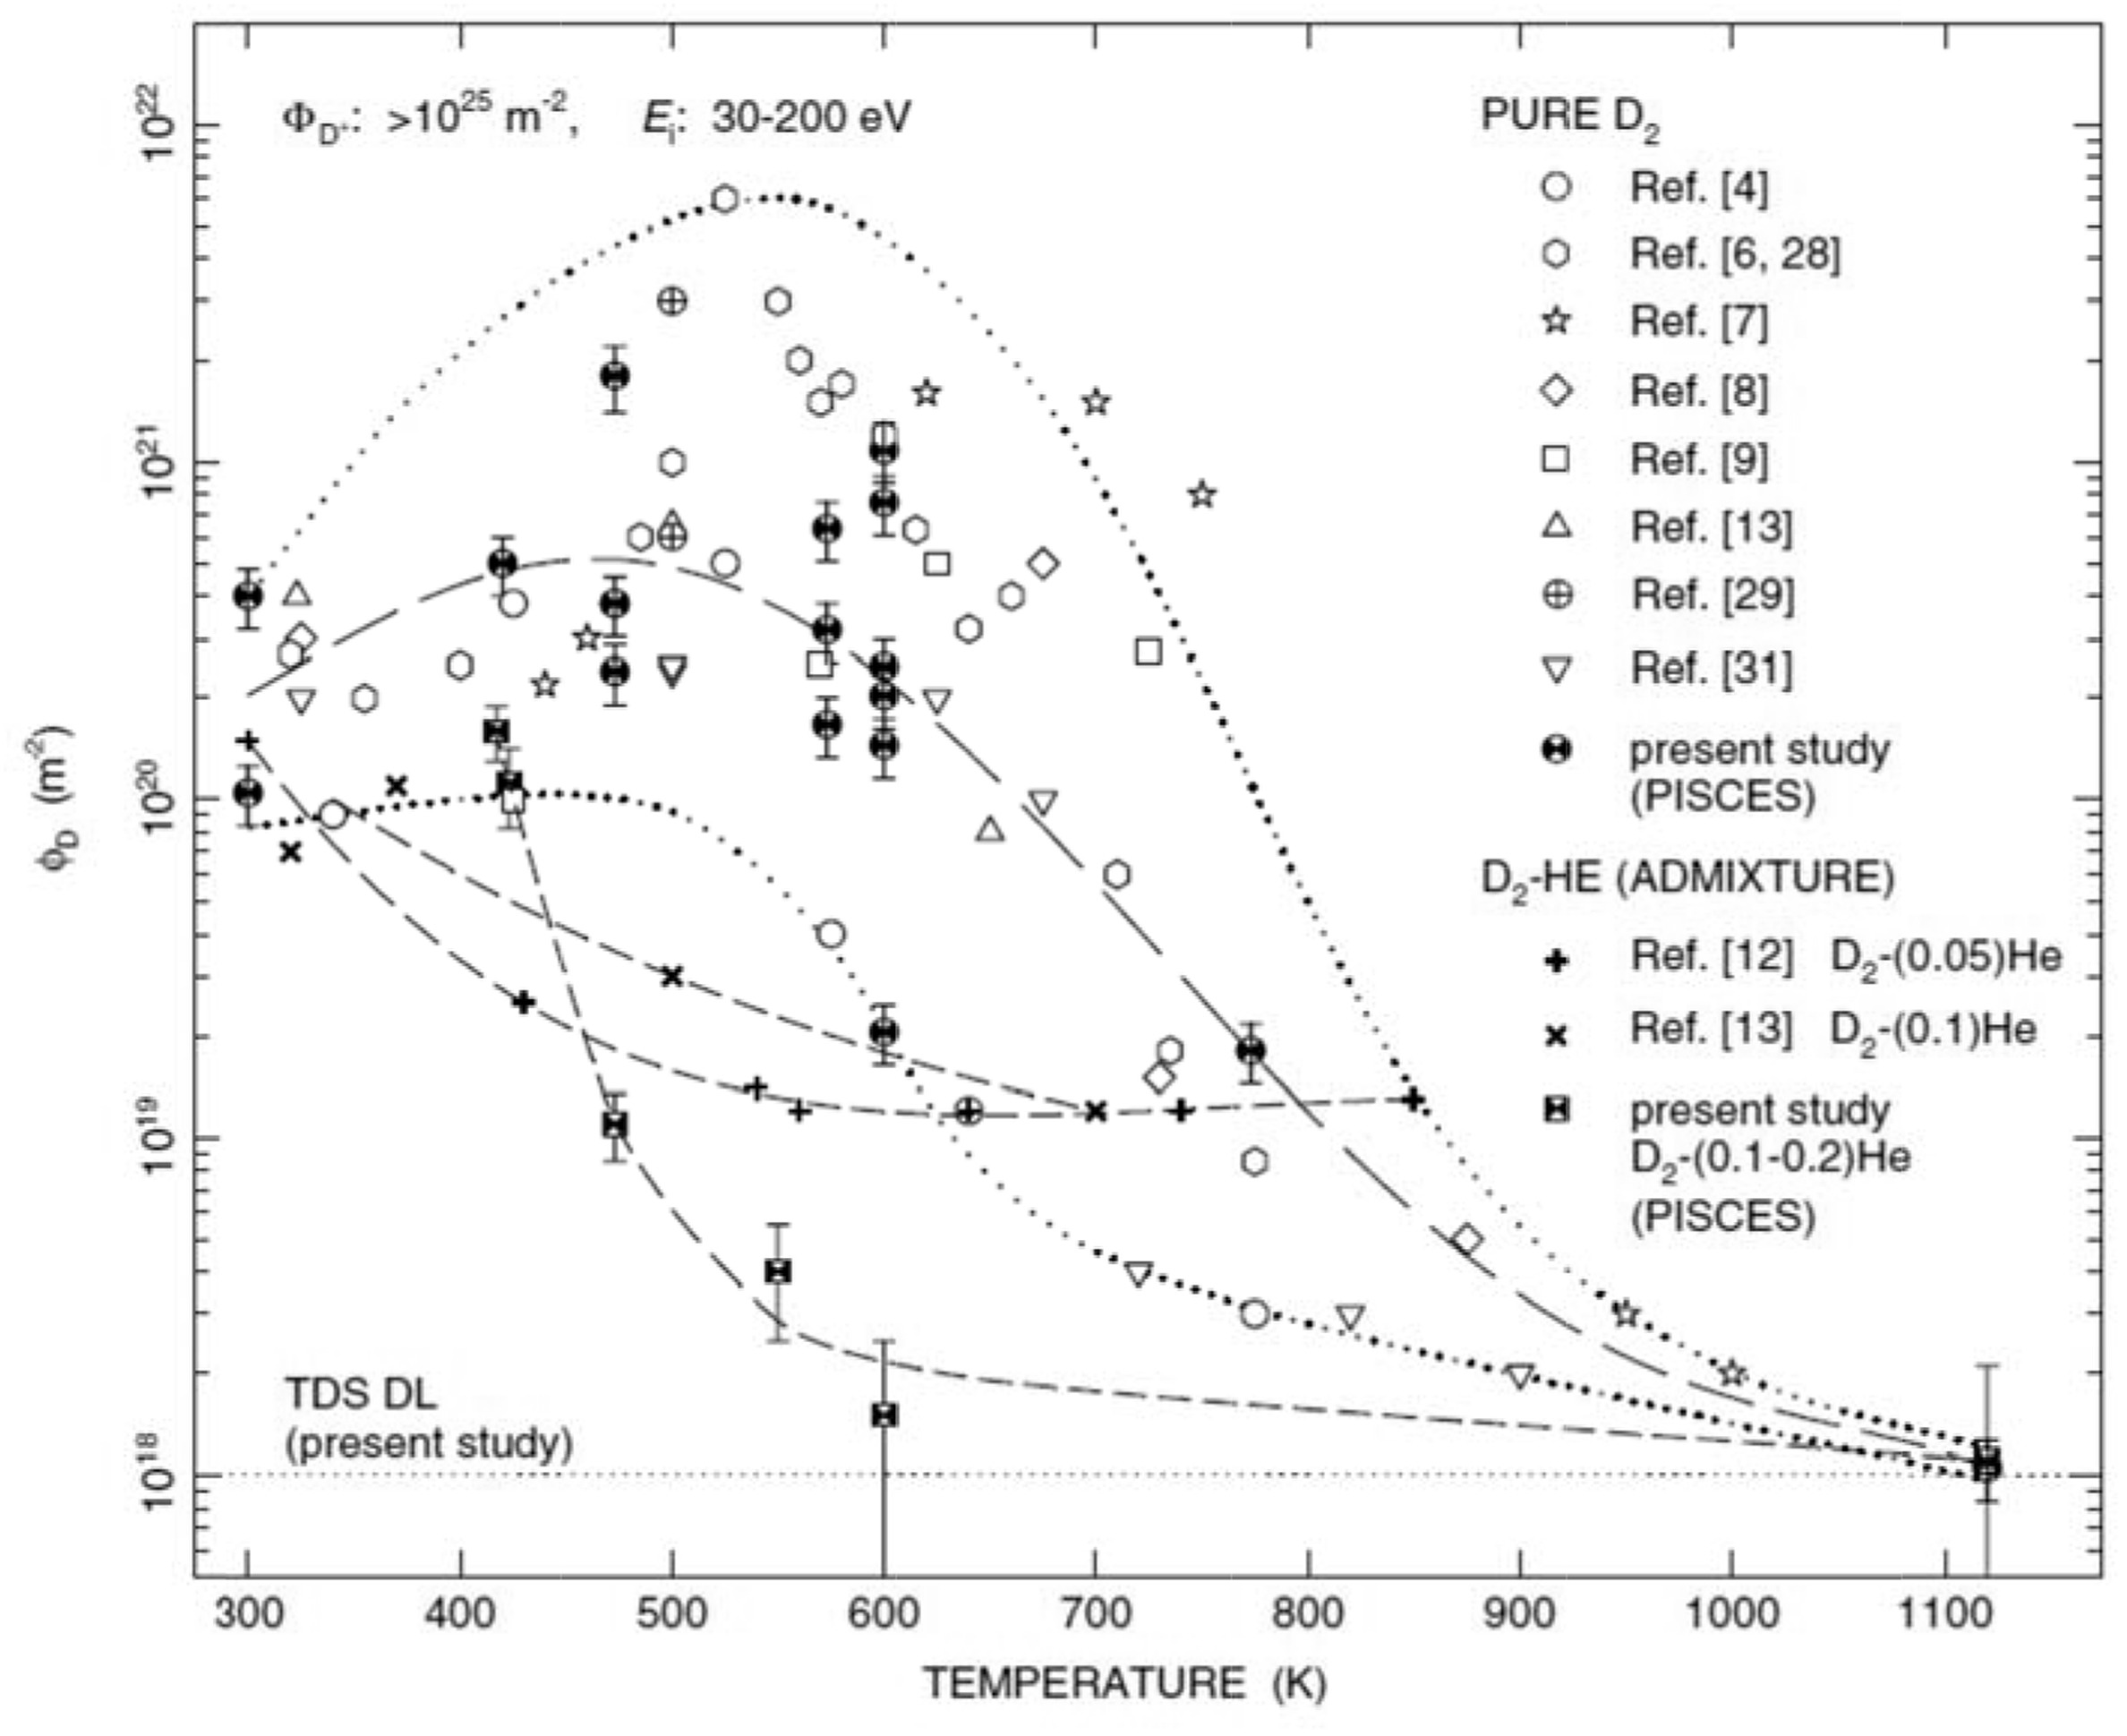
\includegraphics[width=0.49\linewidth]{retention_HeTemperature.png}}
    }
    \caption{Зависимость содержания захваченного дейтерия в вольфраме от а) числа смещений на атом, индуцированных предварительным облучением МэВ-ными ионами~\cite{Roth2011}, и б) температуры~\cite{Rieth2019}}
\end{figure}

Процесс накопления изотопов водорода также сильно зависит от температуры, при которой происходит облучение. Как было показано ранее, процессы диффузии, захвата в дефекты и десорбции протекают интенсивнее при более высокой температуре. В условиях сильного нагрева материала также возможен отжиг имеющихся дефектов, что будет снижать эффективность удержания изотопов водорода~\cite{Dark2024}. Совокупность экспериментальных результатов на рисунке~\cref{fig:ch1/retention_HeTemperature} демонстрирует снижение скорости накопления дейтерия в вольфраме в области температур более \SI{600}{\kelvin}. Примечательно, что интегральное удержание водорода также может быть заметно снижено за счет добавления примеси гелия в поток ионов, что также подавляет образование блистеров на поверхности вольфрама~\cite{Baldwin2011}, 

\subsection{Влияние импульсных нагрузок на накопление}\label{sec:ch1/sec3/subsec4}

Влияние импульсных плазменных нагрузок на накопление изотопов водорода изучено менее детально по сравнению со случаем стационарного облучения. Основной интерес представляют ELM-события, развитие которых ожидается при переходе в режим с повышенным удержанием энергии в плазме токамака. Ранее отмечалось, что ELM-события сопровождаются выбросом горячей плазмы на ОПЭ, создающим импульсно-периодические потоки тепла и частиц в дополнение к стационарным. Полностью воспроизвести такие параметры облучения в лабораторных условиях на данный момент не представляется возможным, поэтому применяются различные подходы по имитации воздействия импульсных нагрузок.

Эксперименты по анализу влияния импульсных тепловых нагрузок во время стационарного плазменного облучения вольфрама ионами дейтерия проводились на установке PSI-2~\cite{Huber2016_1, Huber2016_2}. Облучение проводилось при потоке ионов \SI{6e21}{\Deuterium\per\meter\squared\per\second} с энергией \SI{60}{\electronvolt}. Импульсные тепловой нагрев осуществлялся при помощи лазерных импульсов длительностью \SI{1}{\milli\second} и частотой повторения \SI{0.5}{\hertz} с плотностью мощности в диапазоне \SIrange{0.19}{0.86}{\giga\watt\per\meter\squared}. При совместном плазменном и лазерном воздействии накопление дейтерия в вольфраме увеличивалось в несколько раз по сравнению с только плазменным облучением. В работе предполагается, что увеличение доли накопленного дейтерия происходит из-за эффектов термических ударов, образования блистеров и трещин, а также большей подвижности внедренных атомов дейтерия из-за дополнительного нагрева материала. Противоположная ситуация наблюдалась в моделировании влияния ELM-событий на накопления дейтерия путем решения задачи транспорта~\cite{Hu2015}. В работе влияние ELM-событий было сведено к импульсным изменения температуры поверхности, которые приводили к снижению скорости накопления дейтерия.

Существенное накопления наблюдалось при облучении вольфрамовых образцов импульсными потоками дейтериевой плазмы в линейном плазменном ускорителе КСПУ-Т~\cite{Ogorodnikova}. Плотность энергии в ходе экспериментов варьировалась в диапазоне \SIrange{0.3}{3.7}{\mega\joule\per\meter\squared} при длительности импульса равной \SI{1}{\milli\second}. Количество импульсов достигало 30 при промежутках времени между ними равных 15 минутам, что обеспечивало охлаждение образцов до комнатной температуры. Сравнение результатов экспериментов в режиме с плавлением и без (красные пунктирная и сплошная линии) с данными, полученными при стационарном плазменном облучении (черная линия), приведено на рисунке~\cref{fig:ch1/retention_QSPA}. 
\begin{figure}[ht]
    \centerfloat{
        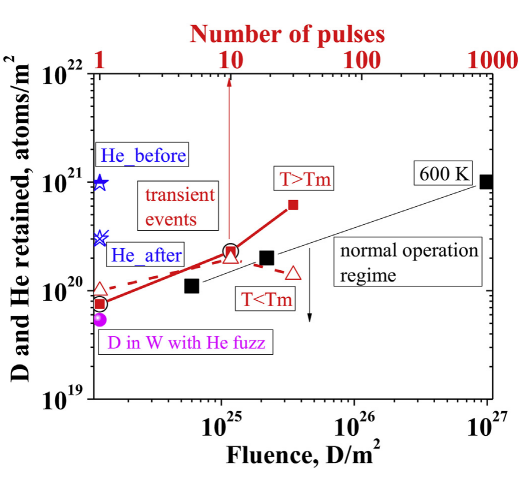
\includegraphics[scale=0.75]{retention_QSPA.png}
    }
    \caption{Зависимость дозы накопленного дейтерия в вольфраме после импульсного плазменного воздействия в режимах без плавления (пунктирная красная линия) и с плавлением (сплошная красная линия) от количества импульсов в сравнении с соответствующей зависимостью после воздействия плазмы в зависимости от дозы облучения~\cite{Ogorodnikova}}\label{fig:ch1/retention_QSPA}
\end{figure}
Существенный захват наблюдается при одном импульсе в обоих режимах. Однако при увеличении числа импульсов в режиме без плавления накопление дейтерия уменьшается. Это, как предполагается в работе, связано с образованием трещин, которые увеличивают площадь свободной поверхности и облегчают десорбцию. В режиме с плавлением, напротив, наблюдается рост накопления дейтерия. Это объясняется более интенсивной диффузией из области расплава в объем вольфрама. Проникновение на большую глубину (\( \sim \SI{10}{\micro\meter} \)) за один импульс было численно продемонстрировано в аналогичной работе~\cite{Poskakalov2020}, в которой также был представлен эмпирический факт о росте доли захваченного дейтерия с увеличением плотности энергии плазменного импульса с \num{0.4} до \SI{3.7}{\mega\joule\per\metre\squared}. Однако абсолютно противоположная ситуация наблюдалась в более ранних экспериментах на установке MCPG~\cite{Nishijima2011}. Вольфрамовые образцы облучались десятью плазменными импульсами длительностью \( \approx\SI{0.5}{\milli\second} \). Исходя из анализа полученных данных, доза захваченного дейтерия уменьшилась более чем в четыре раза при увеличении плотности энергии импульса с \num{0.5} до \SI{0.7}{\mega\joule\per\meter\squared}.

Таким образом, небольшой объем имеющихся экспериментальных данных не позволяет однозначно охарактеризовать влияние импульсных плазменных нагрузок на накопление изотопов водорода в вольфраме. Кроме этого, параметры облучения в лабораторных установках не могут в полной мере воспроизвести условия, характерные для токамаков. Анализ захвата изотопов водорода во время переходных процессов в токамаках проводят путем решения задачи транспорта в ОПЭ, используя параметры облучения, полученные с диагностических зондов, или при совместном моделировании процессов в пристеночной плазме и в объеме. Моделирование накопления в условиях, имитирующих ELM-событиям в токамаке JET, продемонстрировало незначительное снижении скорости накопления дейтерия и флуктуации температуры поверхности с амплитудой \( \approx \SI{100}{\kelvin} \)~\cite{Schmid2016}. В работе также показано, что коэффициент рециклинга быстро достигает и колеблется вблизи единицы. Такая же динамика изменения коэффициента рециклинга наблюдается и в более поздних работах по исследованию влияния развития ELM-неустойчивости в магнитной геометрии токамака DIII-D на основе согласованного моделирования процессов в приповерхностной плазме и ОПЭ~\cite{Lasa2024,Smirnov2024}. Однако также отмечается, что амплитуда колебаний определяется параметрами комбинированного облучения в ходе разряда. Динамическое удержание дейтерия в ОПЭ может играть решающую роль в балансе частиц плазмы на периферии во время ELM-цикла и, следовательно, влиять на время восстановление пьедестала. Расчеты с использование более детальной модели транспорта водорода и экспериментальных параметров облучения не ставили целью анализ динамики интегрального накопления, но показали, что повышение температуры во время ELM-событий приводит к агломерации и повышению концентрации сложных дефектов с более высокой энергией связи в поверхностном слое~\cite{Heinola2019}. Численный анализ динамики удержания с использованием экспериментальных данных токамака EAST, но, по всей видимости, не учитывающий временную эволюцию температуры, продемонстрировал увеличение интегрального накопления примерно на \SI{20}{\percent} во время ELM-событий из-за большей вероятности внедрения быстрых частиц и образования ион-индуцированных дефектов~\cite{Sang2014}.  

\section{Лазерно-индуцированная десорбция дейтерия}\label{sec:ch1/sec4}

Развитие методов анализа содержания изотопов водорода является задачей, непосредственно связанной с вопросом их накопления в элементах вакуумной камеры установки. Глобальные измерения содержания изотопов водорода осуществляются методом газового баланса на основе измерения потоков введенных в камеру и откачанных частиц Различные методы \textit{post-mortem} анализа предоставят информацию о локальном количестве удержанного водорода в извлеченных элементах. Подобные методы анализа предоставляют только данные об интегральном накоплении в ходе кампании и обычно не могут быть использованы для характеризации отдельных плазменных разрядов. Следует отметить, что извлекаемые из вакуумной камеры образцы, как правило, подвергаются воздействию атмосферы во время транспортировки и хранения, что может усложнять интерпретацию результатов измерений.

Осуществление \textit{in situ} анализа возможно при помощи методов, основанных на взаимодействии лазерного излучения с поверхностью внутрикамерных элементов. Применение лазерных методов позволяет проводить локальное пробирование участков поверхности, когда получение информации о пространственных параметрах может быть получено путем сканирования различных областей первой стенки. Среди методов, разрабатываемых для установок с магнитным удержанием плазмы, можно выделить лазерно-индуцированную десорбцию (ЛИД), лазерно-индуцированную абляцию (ЛИА) и лазерно-искровую эмиссионную спектроскопию (ЛИЭС)~\cite{Philipps2013,Mukhin2016}. Схематическое представление каждого из методов приведено на рисунке~\cref{fig:ch1/laser_methods}.
\nomenclature[A, 10]{ЛИА}{Лазерно-индуцированная абляция}
\nomenclature[A, 11]{ЛИЭС}{Лазерно-искровая эмиссионная спектроскопия}
\nomenclature[A, 12]{КМС}{Квадрупольный масс-спектрометр}

\begin{figure}[ht]
    \centerfloat{
        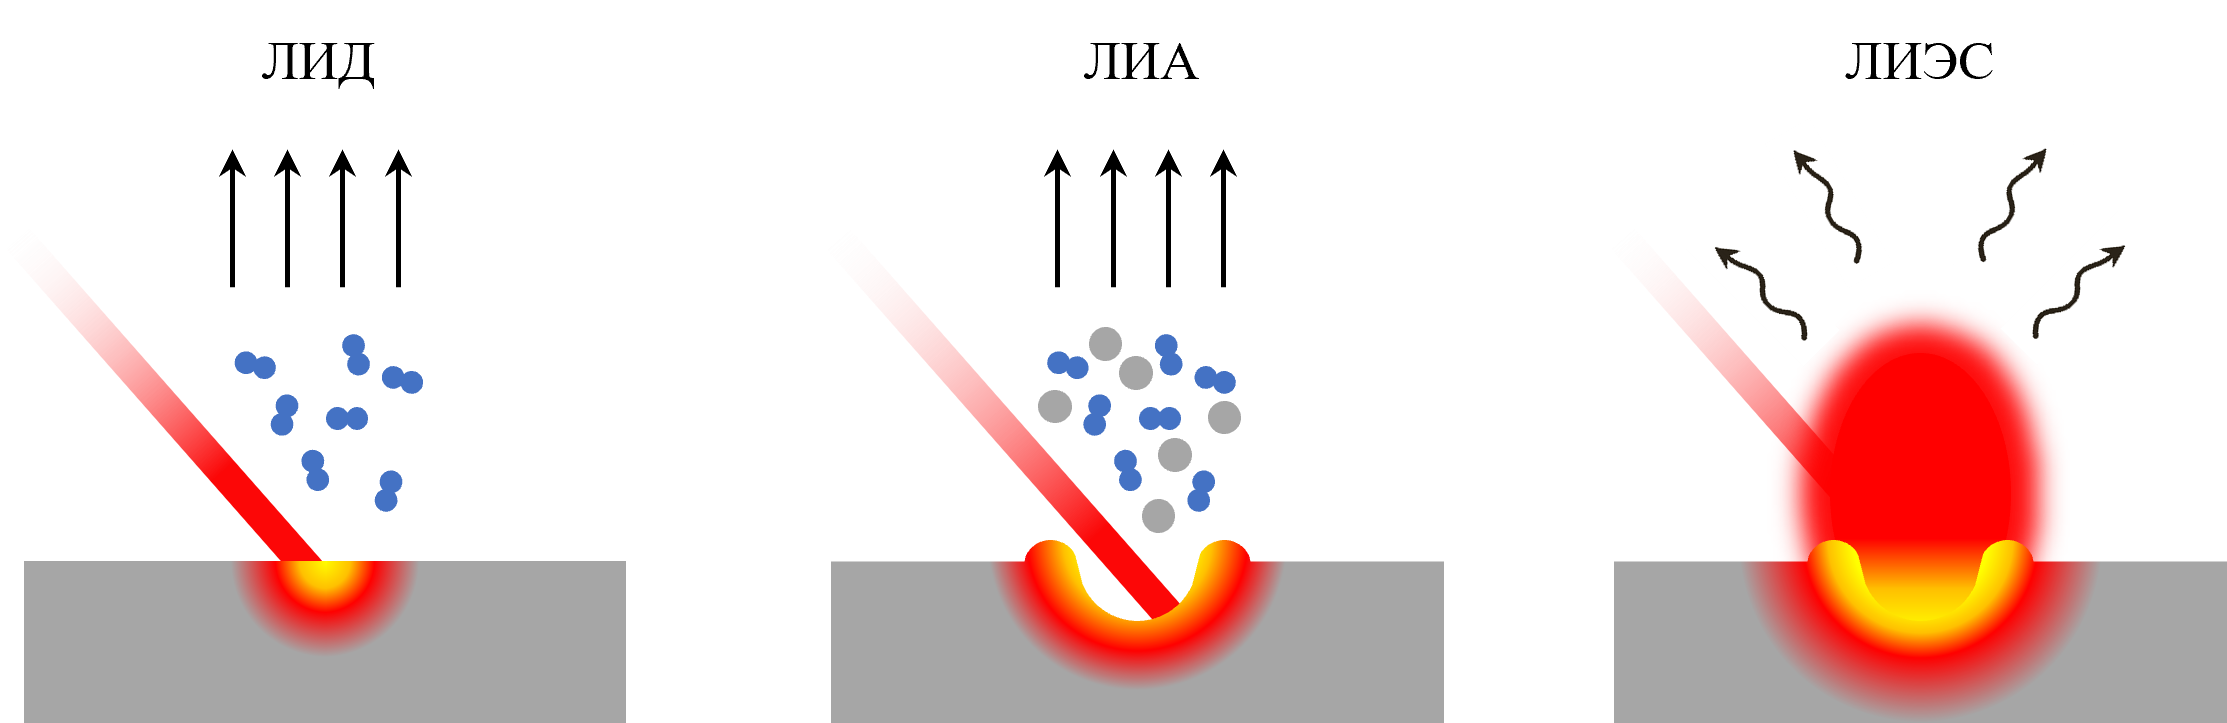
\includegraphics[scale=1]{laser_methods.png}
    }
    \caption{Схематическое представление лазерно-ассистированных методов анализа содержания изотопов водорода в ОПЭ}\label{fig:ch1/laser_methods}
\end{figure}

Основные процессы, лежащих в основе различных методов, можно условно дифференцировать в зависимости от плотности мощности лазерного излучения, но важно заметить, что границы применимости каждого из подходов зависят от материала и состояния поверхности. В ЛИЭС обычно используется интенсивное (\( >\SI{1}{\giga\watt\per\meter\squared} \)) наносекундное лазерное облучение, которое ведет к образованию плазменного факела. Определение состава плазмы происходит на основе спектроскопии эмиттированного излучения. Данная диагностика позволяет проводить анализ по глубине и была апробирована на множестве токамаков~\cite{Xiao2015,Semerok2016,Imran2023,Favre2024}, однако точность интерпретация результатов измерений сильно зависит от параметров образующейся плазмы~\cite{Marenkov2021}. 

ЛИА проходит в промежуточном диапазоне плотности мощности лазерного излучения (\SIrange{0.5}{1.0}{\giga\watt\per\meter\squared}) с наносекундной длительностью и сопровождается только абляцией материала исследуемой поверхности и десорбцией захваченного газа за счет нагрева. Аблированные атомы затем детектируется напрямую квадрупольным масс-спектрометром (ЛИА-КМС) или за счет оптической спектроскопии излучения при ионизации в приповерхностной плазме (ЛИАС). Метод также позволяет проводить анализ содержания по глубине за счет послойной абляции поверхности. ЛИА была успешно применена на таких токамаках, как TEXTOR~\cite{Gierse2016}, EAST~\cite{Hu2018} и Глобус-М2~\cite{Medvedev2024}, демонстрируя перспективность подхода для будущих установок. 

По сравнению с двумя предыдущими диагностиками, ЛИД является неразрушающим и более простым (в плане постобработки) методом, базирующемся на нагреве поверхности. Импульсный нагрев инициирует десорбция захваченных атомов изотопов водорода, которые затем анализируются при помощи КМС (ЛИД-КМС) или оптической спектроскопии (ЛИДС). Применимость ЛИД была продемонстрирована на множестве установок~\cite{Schweer2009, Medvedev2024}, в том числе и на крупном токамаке JET~\cite{, Zlobinski2024}. Учитывая перспективность метода, соответствующие диагностические комплексы разрабатываются для токамака ИТЭР и предложены для токамака ТРТ~\cite{Razdobarin2022}. 

Эффективность ЛИД (доля десорбированных атомом по отношению к их начальному количеству) дейтерия из соосажденных бериллиевых пленок определялась при длительности лазерного нагрева в диапазоне \SIrange{1}{10}{\milli\second}~\cite{Zlobinski2019, Zlobinski2020}. Результаты экспериментов, приведенные на рисунке~\cref{fig:ch1/LID_efficiency}, демонстрируют практически полный выход захваченного дейтерия за один импульс при достижении температуры плавления бериллия. 
\begin{figure}[ht]
    \centerfloat{
        \hfill
        \subcaptionbox[List-of-Figures entry]{\label{fig:ch1/LID_efficiency_thin}}{%
            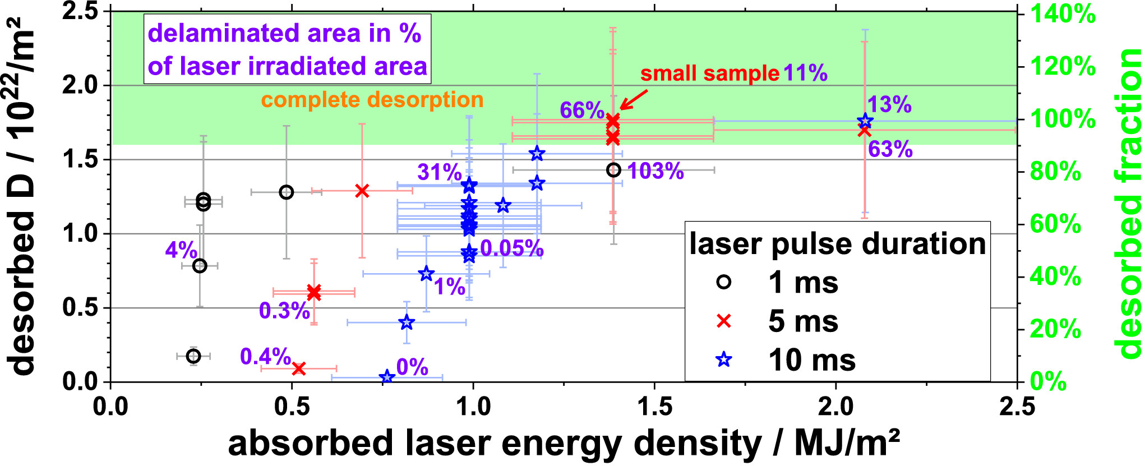
\includegraphics[width=0.49\linewidth]{LID_efficiency_thin.png}}
        \hfill
        \subcaptionbox{\label{fig:ch1/LID_efficiency_thick}}{%
            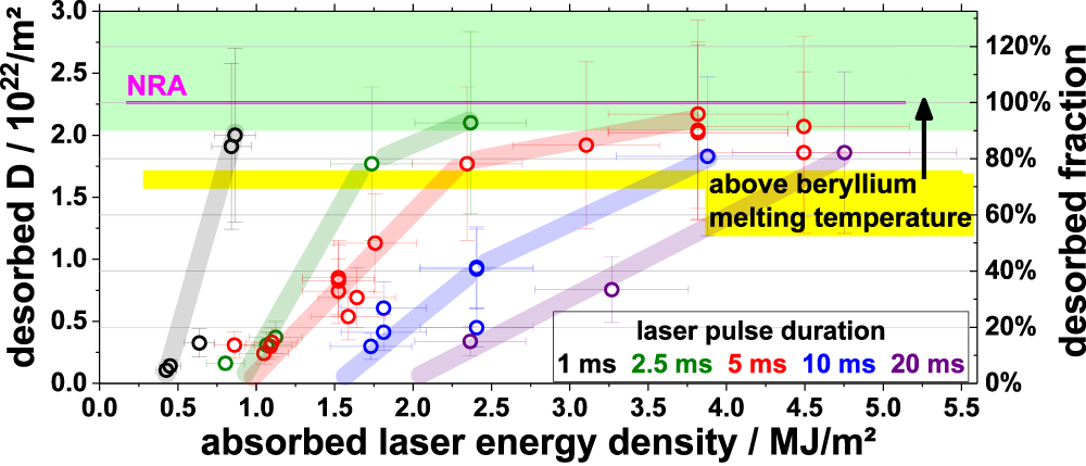
\includegraphics[width=0.49\linewidth]{LID_efficiency_thick.png}}
    }
    \caption{Зависимость числа десорбированных атомов дейтерия из соосажденных пленок бериллия от плотности поглощенной энергии лазерного импульса различной длительности: а) толщина пленки \SI{1}{\micro\meter}, содержание дейтерия \SIrange{25}{30}{\text{ат.}\percent}~\cite{Zlobinski2019}; б) толщина пленки \SI{10}{\micro\meter}, содержание дейтерия \SI{1}{\text{ат.}\percent}~\cite{Zlobinski2020}}\label{fig:ch1/LID_efficiency}
\end{figure}
Применение более длительных импульсов (\SI{1}{\second}) при анализе эффективности десорбции дейтерия из соосажденных пленок вольфрама (толщина \SI{1.2}{\micro\meter}, содержание дейтерия \( \approx \SI{1.7}{\text{ат.}\percent} \)) показало эффективность десорбции на уроне \SI{97}{\percent} за один импульс~\cite{Yu2019}.

Высокая эффективность дегазации толстых пленок, образование которых возможно при распылении материалов ОПЭ во время длительных плазменных разрядов в ТЯУ, говорит о необходимости использования более долгих лазерных импульсов для определения интегрального накопления в них. Рассматривается также возможность использования наносекундных лазерных импульсов для ЛИД~\cite{Medvedev2024, Gasparyan2021, Efimov2024}. При таком воздействии глубина прогрева материала составляет \SIrange{50}{100}{\nano\meter}, что позволяет анализировать тонкий поверхностный слой. В то же время, возможной становится реализация режима ЛИА. Объединение нескольких методов диагностики в рамках одного комплекса расширяет возможности анализа, а также облегчает проектирование и распределение компонентов крупных установок типа токамак.

Открытым остается вопрос о влияние параметров материала и центров захвата изотопов водорода в нем на эффективность ЛИД. Известно, что структура соосажденных слоев отличается от идеальной кристаллической. Помимо этого, в условиях, характерных для ТЯУ, будет происходить непрерывная эволюция параметров дефектов, определяющих удержание изотопов водорода. Соответственно, исследование закономерной выхода изотопов водорода из материалов ОПЭ актуально для определения эффективных режимов и оценки возможных источников погрешности ЛИД. 

\section{Выводы к главе 1}

Совокупность физических свойств вольфрама определяет перспективность его использование для элементов облицовки ТЯУ. В настоящее время он выбран в качестве основного материала ОПЭ токамака ИТЭР. Оценки накопления радиоактивного трития в ИТЭР не учитывают в полной мере весь спектр процессов, протекание которых ожидается при достижении проектных параметров установки. 

Существенным пробелом является отсутствие однозначной информации о влияние импульсных плазменных нагрузок во время быстрых переходных процессов, как ELM-события, сопровождаемых переход в режим с улучшенным удержанием энергии в плазме токамаков. Проблема усугубляется технической сложностью реализации импульсных плазменных нагрузок, релевантных условиям в масштабных установках, как ИТЭР. 

На большинстве современных токамаках идет активная разработка и апробация методов дистанционного контроля содержания изотопов водорода. Среди них, лазерно-индуцированная десорбция является перспективным методом, позволяющим проводить анализ содержания без нанесения существенного ущерба поверхности. Исследование закономерностей выхода изотопов водорода при лазерном нагреве актуально для определения наиболее эффективных режимов диагностики и определения возможных источников погрешности.


\FloatBarrier
